\section{Formalización del problema}


\subsection{Exploración}
La exploración de un entorno desconocido es problema clásico de la robótica móvil que consiste en utilizar un robot con el objetivo de obtener información de un entorno desconocido con el propósito de generar un mapa que lo represente. La exploración es fundamental en tareas de búsqueda y rescate \cite{Liu2015} y misiones extra planetarias \cite{schuster2019towards}, tareas normalmente llevadas a cabo en escenarios donde puede ser ineficiente o directamente inviable teleoperar a un robot. Por lo tanto que el robot pueda explorar el entorno de forma autónoma es una característica deseable.

Uno de los principales aspectos de la exploración autónoma es el problema de la asignación de tareas de exploración que suele separarse en dos partes principales, (i) identificar posibles objetivos de exploración y (ii) asignar al robot a una de dichos objetivos \cite{amorin2019novel}. Para determinar potenciales objetivos de exploración, un método popular es el propuesto en \cite{yamauchi1998frontier} que consiste en identificar las fronteras entre el espacio conocido y desconocido, y utilizarlas como potenciales objetivos. Asignar un robot a uno de los posibles objetivos consiste en determinar cual de estos es el mas conveniente, para esto se suele hacer un balance entre el costo y el beneficio de completar el objetivo. El costo normalmente involucra aspectos como la distancia del recorrido que el robot debe hacer para llegar al objetivo, y cual será dificultad de recorrerlo, por otro lado beneficio usualmente se asocia al tamaño de la porción explorada al completar el objetivo. 

\subsection{Exploración multi-robot}\label{subsec:expmutirob}
La exploración multi-robot consiste en utilizar una flota robótica para resolver el problema de la exploración, por las razones antes mencionadas la exploración multirobot autónoma es de interés.  

Una de las ventajas de utilizar varios robots es la introduce redundancia, aumento la tolerancia a fallos que esto implica. A su vez la exploración suele ser altamente paralelizable, al ser usual que en un mismo instante de tiempo hallan varios lugares en los cuales un robot puede obtener información, por lo que es esperable que al aumentar la cantidad de recursos roboticos se experimente una reducción los tiempos de exploración \cite{cao1997cooperative}, \cite{dudek1996taxonomy}, \cite{guzzoni1997many}. 

Sin embargo el aumento del numero de robots en una flota de exploración no es proporcional a la reducción de tiempo de exploración. En primer lugar el numero de objetivos es finito durante todo el proceso de exploración, siempre que el numero de robots sea mayor a el numero de objetivos de exploración, se tendrá recursos desaprovechados. De forma similar si varios robots son enviados a objetivos de exploración cercanos entre si existe la posibilidad de que los sensores que estos utilizan para explorar recolecten información sobre una misma parte del entorno y por lo tanto realicen trabajo redundante. Adicionalmente al existir un mayor numero de robots aumenta el riesgo de que estos se interfieran entre si, causando perdidas de tiempo en desvíos para evitar colisiones \cite{guzzoni1997many}, \cite{goldberg1997interference}. %% Esto determina que existe un numero optimo de robots en una flota, en el cual se logra un balance entre la capacidad de explotar el paralelismo en la exploración y el tiempo perdido por interferencias. 
Las problemáticas mencionadas pueden ser mitigadas realizando la asignación de objetivos debe se de forma coordinada buscando explotar el paralelismo en la exploración y reducir el tiempo perdido por interferencias \cite{nieto2014coordination}. Básicamente, la exploración coordinada consiste en resolver el problema de la asignación de tareas de forma de que se maximice la relación costo-beneficio, no de un solo robot, si no que de la flota entera.

 % que consiste en asignar los robots a objetivos de exploración de forma inteligente 

% El numero optimo mencionado coordinación que logre evitar interferencias suele ser un factor critico en la exploración multirobot porque permite lograr el balance anteriormente mencionado con una cantidad de robots mayor al que se podría tener sin coordinar\cite{nieto2014coordination}.


% Los probas anteriormente mencionados pueden ser mitigados con el uso de una buena estrategia de coordinación.



% No se bien si esta sección va como parte del estado del arte o seria parte de la intro. Algunas cosas que se pueden incluir en esta son:

%   Descripción genérica del problema

%   Aspectos a considerar
  
%   Problemas relacionados

%   Soluciones posibles a alto nivel

\subsection{Mapas}\label{subsec:mapas}
Un mapa consiste en un modelo de un entorno, en el contexto de la robótica los mapas se pueden dividir en dos categorías, \emph{mapas métricos} y \emph{mapas topológicos} \cite{Thrun1998}, \cite{choset2005principles}.

Los \emph{mapas métricos} son mapas principalmente caracterizados por representar la geometría de todo el entorno, incluyendo a su vez una escala que permite asociar las dimensiones representadas dentro del mapa con las dimensiones reales.

Un tipo de mapa métrico es el denominado \emph{mapa geométrico}, en estos se utilizan primitivas geométricas para representar al entorno, aunque es usual el uso de segmentos de recta como primitiva, es posible utilizar otras primitivas de ser conveniente. Un ejemplo de este tipo de mapa se puede ver en la figura \ref{fig:ejMapMetrico}, siendo las primitivas utilizadas rectángulos.

Una \emph{grilla de ocupación} es un tipo de mapa métrico que se basa en una teselación del espacio en celdas que conforman una grilla donde cada celda almacena una estimación probabilística de su estado (libre u ocupado). En la figura \ref{fig:ejGrillaOc} se muestra una grilla de ocupación en la que cada celda se encuentra coloreada según su probabilidad de encontrarse en un estado ocupado o libre, los colores oscuros indican una mayor probabilidad del estado ocupado y los mas claros una mayor intensidad de estar libres.

Los \emph{mapas topológicos} por otro lado son mapas simplificados al punto de solo incluir lugares topológicamente distintivos y conexiones entre estos. Normalmente se representan con grafos donde las lugares son los vertices y las aristas son las conexiones entre ellas. Dependiendo del contexto es posible que los mapas topológicos contengan información adicional en los vertices y aristas.

Los tipos de mapas topológicos se determinan según lo representado por un vértice, en los \emph{mapas topológicos basados en regiones} los vertices corresponden a regiones de interés resultantes de una segmentación del espacio que corresponden a habitaciones y corredores en entornos estructurados como lo son las casas y oficinas. La figura \ref{fig:ejMapTop} es un ejemplo de un mapa topológico basado en regiones. Notar que en este ejemplo, para que fuera mas ilustrativo, los vertices del grafo utilizado como representación fueron dispuestos para que coincidan con su correspondiente ubicación en el entorno, pero el grafo no tiene porque contener la información necesaria para esto.

\begin{figure}[H]
  \centering
  \subfloat[Mapa geometico]{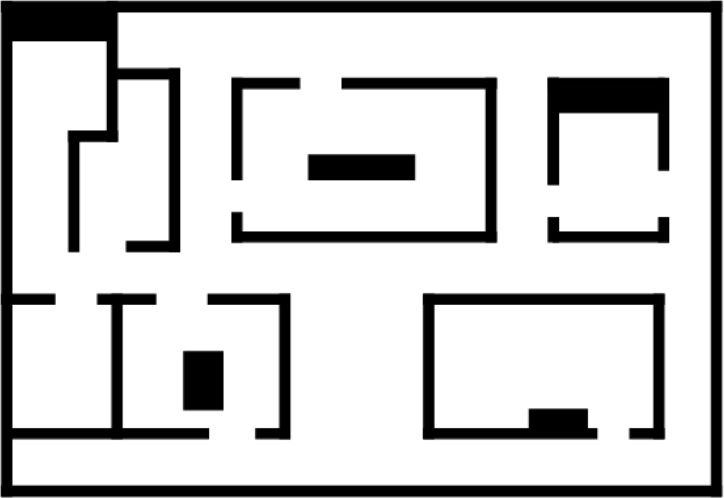
\includegraphics[clip=true, width=0.29\linewidth]{imagenes/tiposDeMapa/metrico.png}\label{fig:ejMapMetrico}}
  \qquad
  \subfloat[Grilla de ocupacion]{
\includegraphics[clip=true, width=0.29\linewidth]{imagenes/tiposDeMapa/grillaDeOc.png}\label{fig:ejGrillaOc}}
  \qquad
  \subfloat[Mapa topologico basado en regiones]{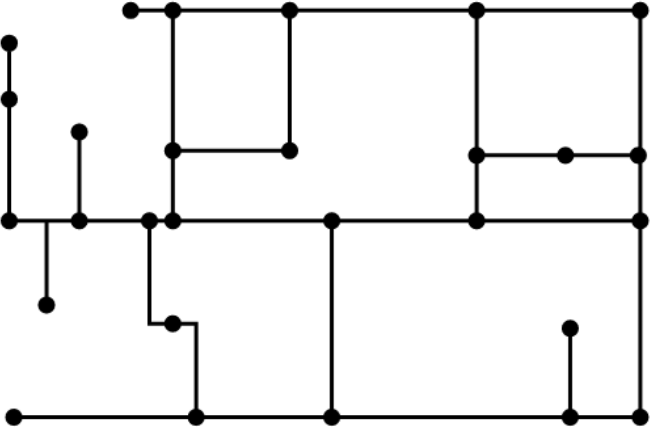
\includegraphics[clip=true, width=0.29\linewidth]{imagenes/tiposDeMapa/topologico.png}\label{fig:ejMapTop}}
  \caption{Un mismo entorno representado con distintos tipos de mapas. Extraído de \cite{choset2005principles}.}
\end{figure}


La simplicidad de los mapas topológicos es útil para nosotros los humanos al facilitar la comprensión un entorno y como navegar en el, por lo que es usual ver mapas topológicos de sistemas de transporte (ver figura \ref{fig:metroBsAs}), adicionalmente posibilita instrucciones que nos resultan naturales, por ejemplo, \say{ir a la habitación A}.

\begin{figure}[H]
  \center
  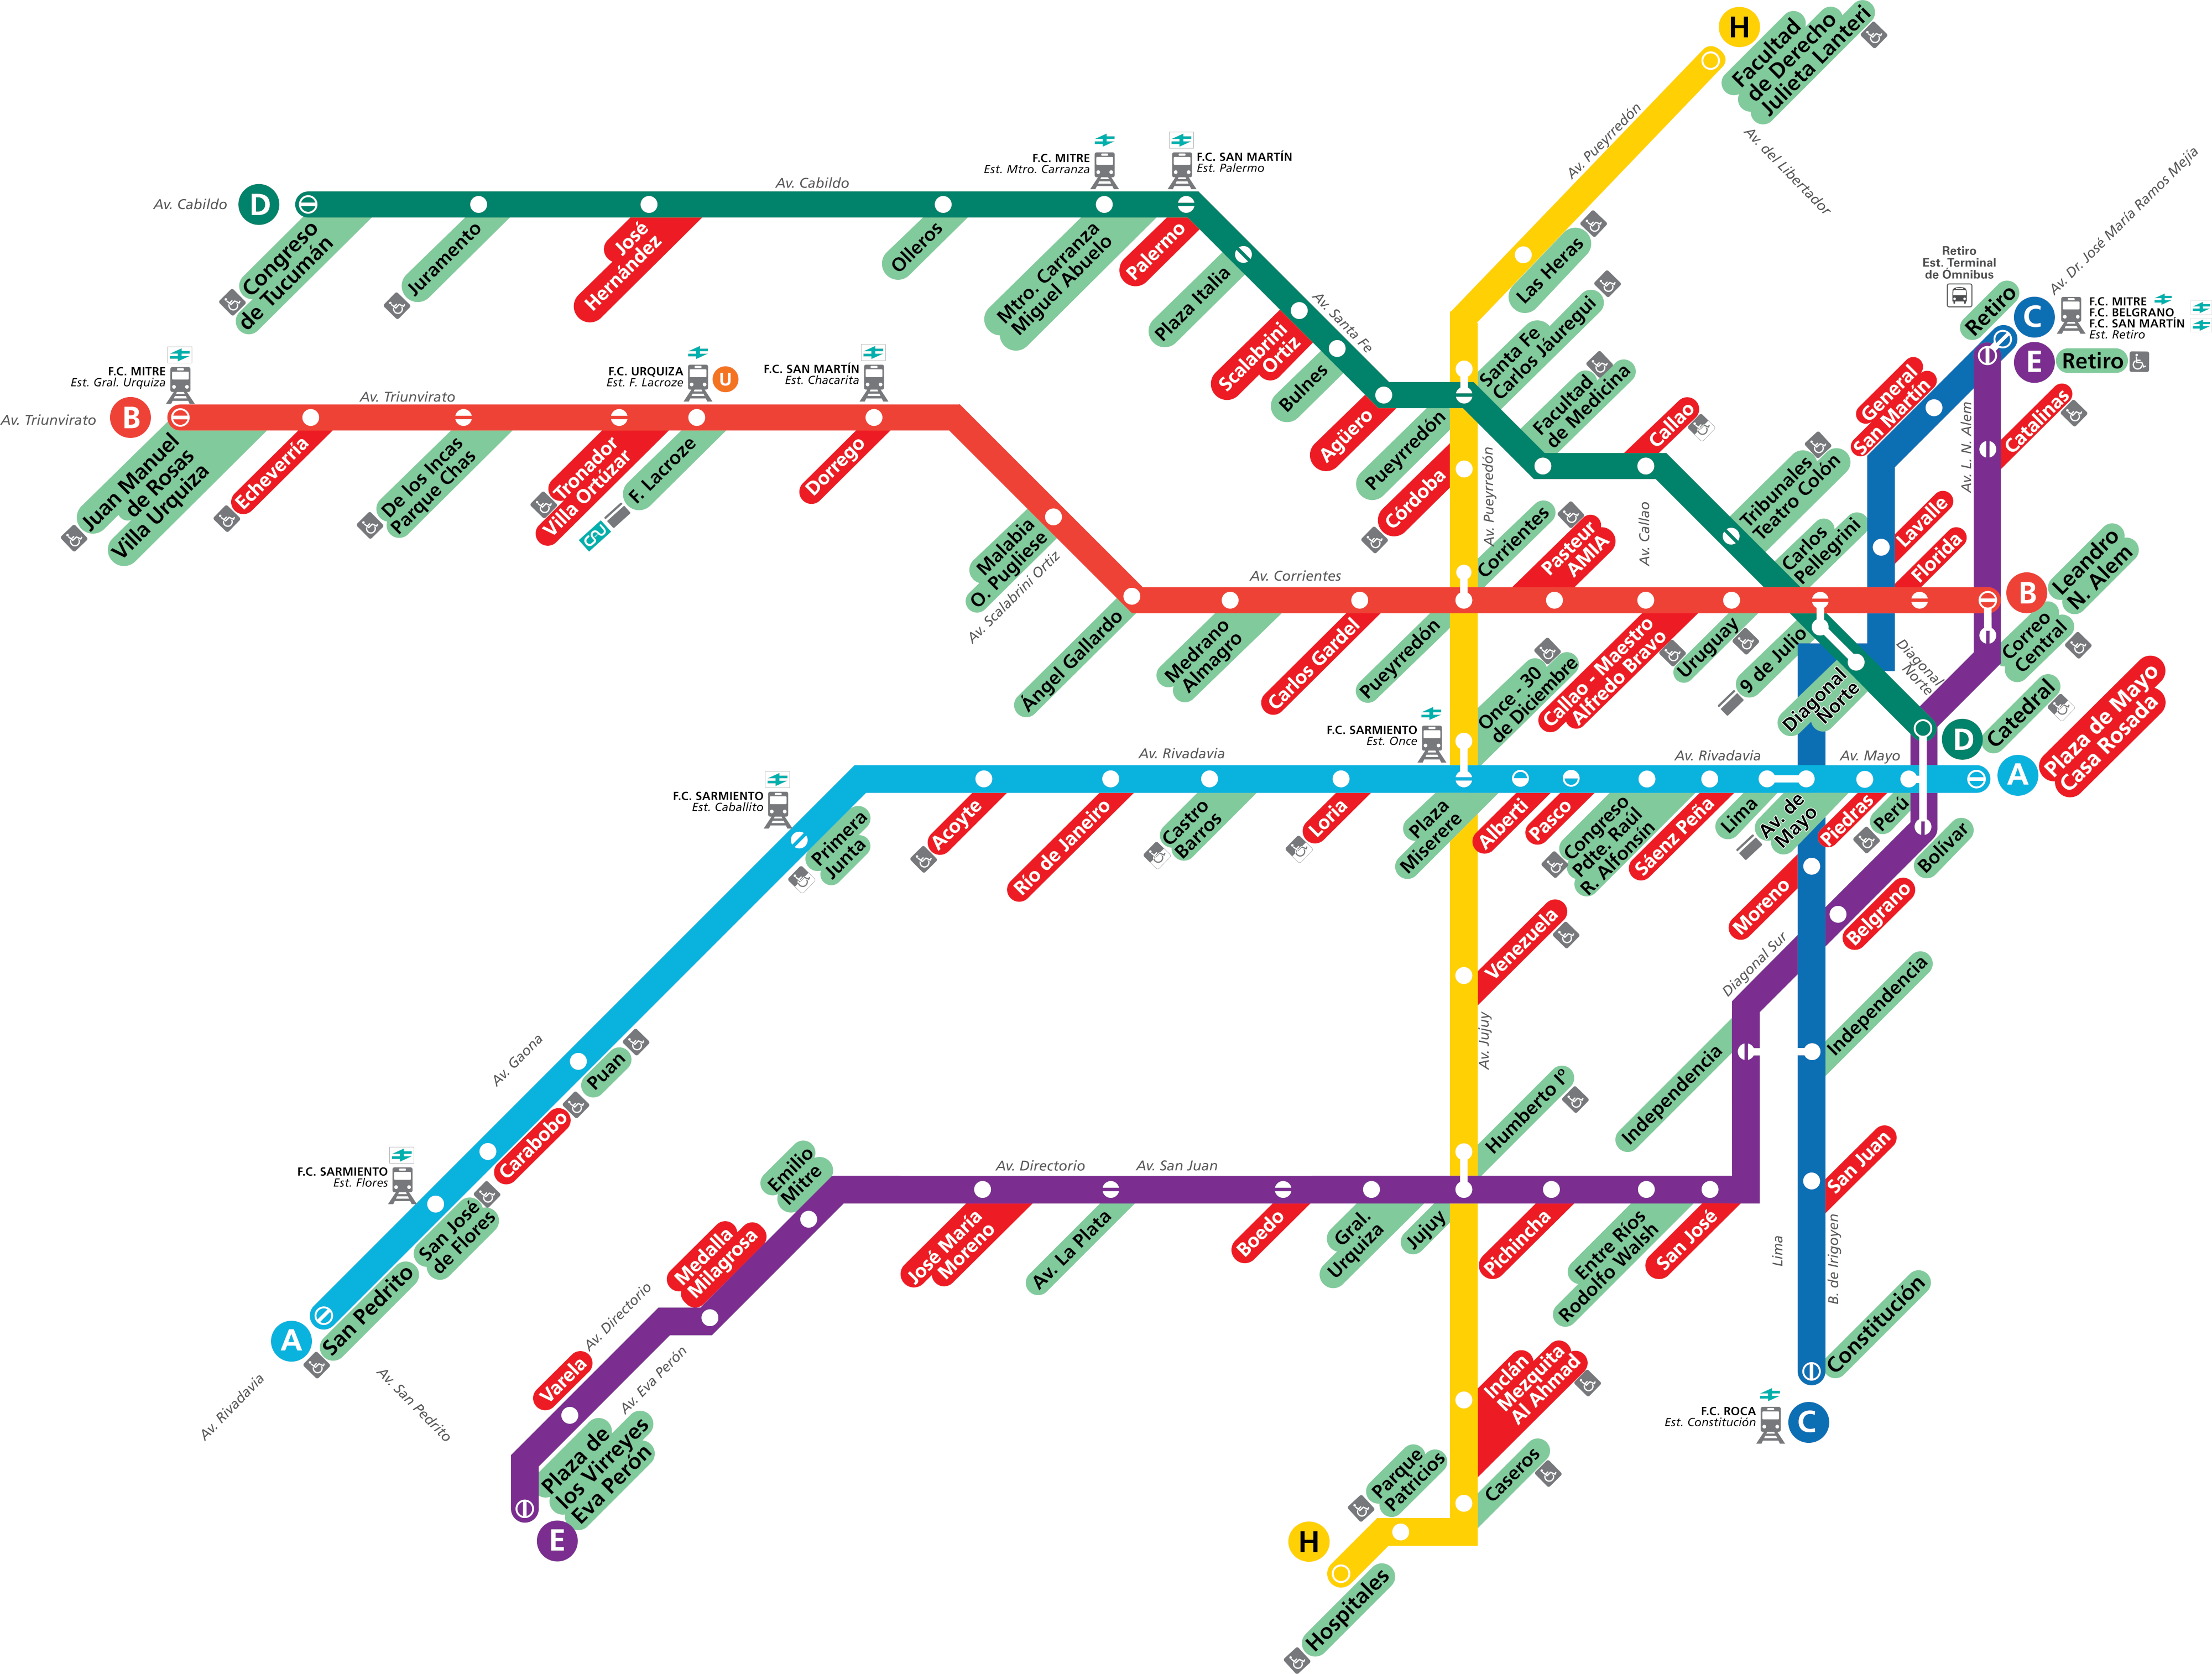
\includegraphics[width=1\linewidth]{imagenes/metroBsAs.png}
  \caption{Mapa de sistema de transporte subterráneo de Buenos Aires, Argentina. Extraído de \cite{metroBsAs}.}\label{fig:metroBsAs}
\end{figure} 

La simplicidad mencionada también tiene ventajas computacionales,  ya que para un mismo entorno los mapas topológicos suelen ser varios ordenes de magnitud mas pequeños que los mapas métricos y por lo tanto, mas allá de la memoria que se ahorra también se tiene una planificación mas eficiente. Sin embargo la falta de detalle en la representación también pude ser una desventaja en tanto hace que los planes de navegación obtenidos de un mapa topológico suelan ser peores que los obtenidos en mapas métricos.

Dadas las ventajas y desventajas mencionadas existen trabajos \cite{Thrun1998}, \cite{wurm2008coordinated}, \cite{Liu2015} que proponen el uso simultaneo de mapas topológicos y métricos para \say{ganar lo mejor de los dos mundos} al tener disponible abstracción y detalle a la vez. Un ejemplo de como combinar las ventajas de ambos tipos de mapa es la planificación jerárquica descrita en \cite{Thrun1998} donde los mapas topológicos son utilizados para generar un plan de navegación topológico que consiste en una secuencia de corredores y habitaciones que se deben atravesar para llegar al objetivo, plan que aunque es fácil de generar no posee suficiente detalle como para traducirse directamente a acciones que el robot pueda realizar para llegar al objetivo. Por lo tanto se introduce una segunda etapa de planificación que consiste en a partir de la grilla de ocupación generar planes métricos que permitan al robot moverse entre los segmentos que componen al plan topológico. De esta forma se evita planificar sobre grilla de ocupación entera y así evitar una gran parte del costo computacional.

Los tres trabajos antes mencionados aunque cada uno tiene sus aportes particulares, tienen en común que el uso de mapas topológicos y métricos a la vez se logra construyendo una grilla de ocupación a partir de los datos obtenidos de los sensores, para luego a partir de la grilla de ocupación generar una estructura intermedia llamada \emph{grafo generalizado de Voronoi} a partir del cual es posible detectar los segmentos que compondrán a un mapa topológico basado en regiones. Este proceso es una parte fundamental del trabajo desarrollado y se detallará a lo largo de las siguientes secciones.

% 
% En esta sección se debe tratar:

% que es una grilla de ocupación.

% Para que sirve en general

% Se puede construir un GVD a partir de una grilla de ocupación. (quizás después?)

% \subsection{Representación poligonal}
% Las representaciones poligonales son mapas métricos propuestos como alternativas a las grillas de ocupación, que busca

\subsection{Mapa de carreteras}\label{subsec:mapacarr}
% Un \emph{mapa de carreteras} (del ingles road map) \cite{choset2005principles} es clase particular de mapas topológicos. Que un mapa topológico cumpla con las condiciones necesarias para ser un mapa de carreteras asegura que a partir de este es posible planificar un camino entre dos puntos cualquiera del espacio libre. La idea detrás de esta categoría esta inspirada por como los humanos utilizamos las redes de carreteras. Al planificar un camino entre dos ubicaciónes distantes, por ejemplo dos depatamentos distintos, en lugar de considerar cada camino posible, normalemte planificamos primero un camino hacia una red de carreteras, luego a lo largo de la red de carreteras y, finalmente, desde la red de carreteras hacia el destino. %(ver figura \ref{fig:ejemplovial}). 
Un \emph{mapa de carreteras} (del ingles road map) \cite{choset2005principles} es clase particular de mapas topológicos. Que un mapa topológico cumpla con las condiciones necesarias para ser un mapa de carreteras asegura que a partir de este es posible planificar un camino entre dos puntos cualquiera del espacio libre. La idea detrás de esta categoría esta inspirada por como los humanos utilizamos las redes de carreteras. Al planificar un camino entre dos puntos distantes, por ejemplo ubicados en dos departamentos de Uruguay: Montevideo y Paysandú, en lugar de considerar cada camino posible, normalmente planificamos primero un camino hacia una red de carreteras (Ruta 1), luego a lo largo de la red de carreteras (a través de ruta 1 y ruta 3), para finalmente, desde la red de carreteras (Ruta 3) ir hacia el destino(ver figura \ref{fig:ejemplovial}). 

\begin{figure}[H]
  \center
  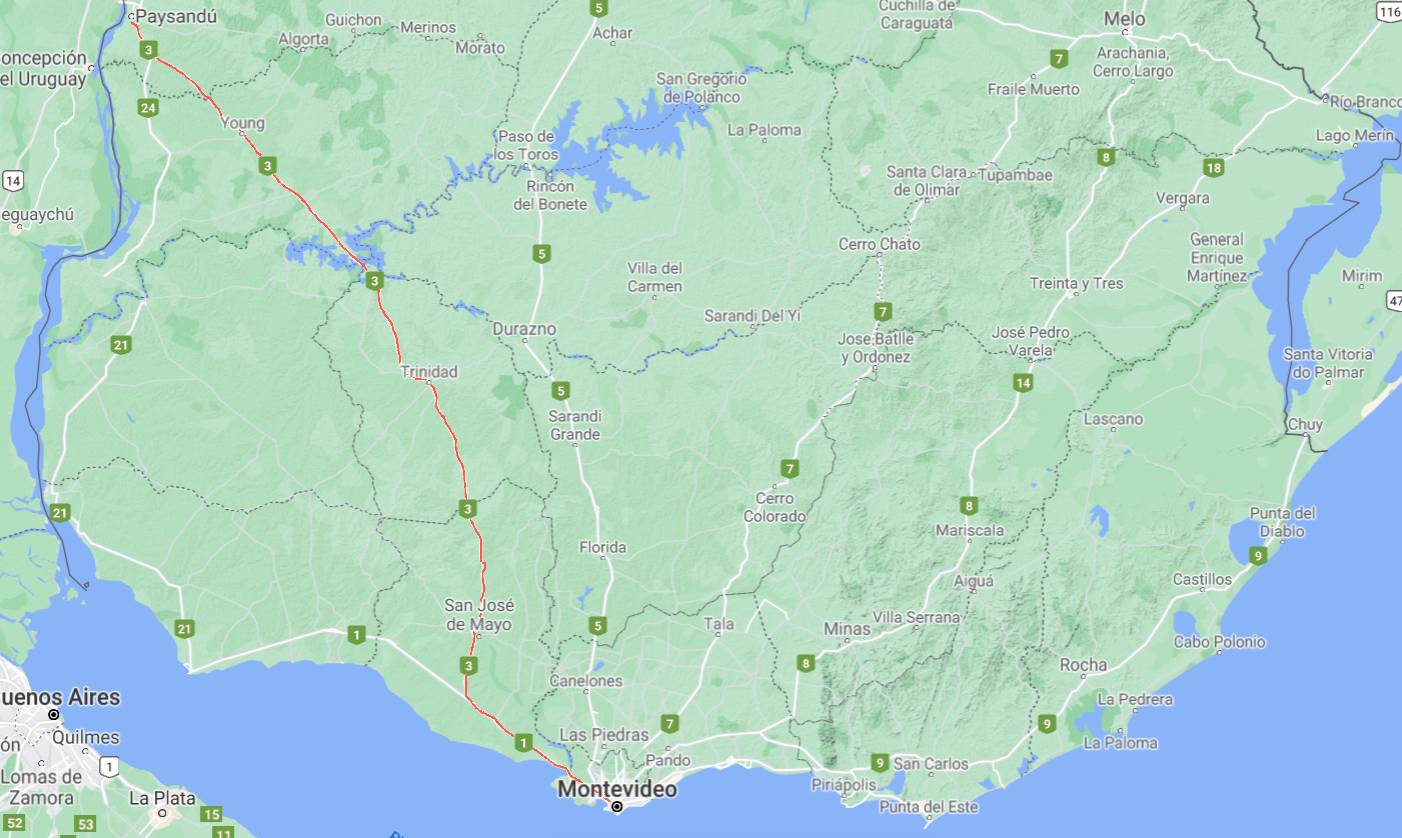
\includegraphics[width=0.9\linewidth]{imagenes/uruguayvialMarcado.png}
  \caption{Mapa de carreteras de Uruguay, con amarillo se resalta un camino entre ubicaciones de Montevideo y Paysandú. Extraído de \cite{googlemaps}.}\label{fig:ejemplovial}
\end{figure} 

Para considerarse un mapa de carreteras, un mapa topológico debe estar representado con un grafo en el cual sus vertices corresponden a puntos no obstaculizados del entorno y sus aristas implican la existencia de caminos disjuntos entre los vertices. Adicionalmente, dicho grafo debe cumplir con 3 propiedades fundamentales, a partir de las cuales es posible asegurar que se puede planificar caminos a partir del mapa de carreteras. Sea $W$ el entorno, $W_{libre} \subset W$ el espacio libre del entorno, y  un grafo $\mli{MC}$, las tres propiedades son:

\begin{enumerate}
  \item Accesibilidad: Para todo $p_{inicio} \in W_{libre}$ existe un camino a un $p'_{inicio}$ vertice de $\mli{MC}$.
  \item Conectividad: Existe un camino entre cualquier par vertices de $\mli{MC}$ $p'_{inicio}$ y $p'_{fin}$.
  \item Capacidad de salida: Para todo $p'_{fin}$ vertice de $\mli{MC}$ existe un camino a un $p_{fin} \in W_{libre}$.
\end{enumerate}

Estas propiedades aseguran la navegación, porque que dados dos puntos $p_{inicio},p_{fin}\in W_{libre}$ es posible construir un camino entre ellos. Primero por \emph{accesibilidad} se tiene un camino entre $p_{inicio}$ y un $p'_{inicio}$ vertice de $\mli{MC}$, luego por \emph{capacidad de salida} se asegura la existencia de un  $p'_{fin}$ vertice de $\mli{MC}$ desde el cual hay un camino a $p_{fin}$ y finalmente por \emph{conectividad} se sabe que existe un camino entre $p'_{inicio}$ y $p'_{fin}$. Entonces uniendo los caminos $p_{inicio} - p'_{inicio}$ (por accesibilidad), $p'_{inicio} - p'_{fin}$ (por conectividad) y $p'_{fin} - p_{fin}$(por capacidad de salida) se tiene un camino que conecta dos puntos genéricos del espacio libre $p_{inicio}$ y $p_{fin}$.

% \cite{choset2005principles}, \cite{Thrun1998}, \cite{Liu2015}.
\subsection{Diagrama de Voronoi}
Dado un espacio $W \subseteq R^2$, $S \subset W$ es un conjunto de puntos llamados \emph{sitios}. Sea $p\in W$, la función $d_p : W \rightarrow R$ computa la distancia entre dos puntos en $W$. Una \emph{region de Voronoi} $R_i\subset W$ es el conjunto de puntos mas cercanos a un sitio $s_i\in S$ particular. %(ecuación \ref{eq:regV})
\begin{equation}
  R_i = \{p \in W : d_p(s_i) \leq d_p(s_j), s_i,s_j\in S,s_j \neq s_i\}\label{eq:regV}
\end{equation}
De forma similar $BP_p \in S$ es el conjunto de sitios mas cercanos a un punto $p \in W$ denominados \emph{puntos bases} de $p$. %\ref{eq:bases} 
\begin{equation}
  \mli{BP}_p =\{s_i : d_p(s_i) \leq d_p(s_j), s_i,s_j\in S,s_j \neq s_i\}\label{eq:bases}
\end{equation}
Un \emph{diagrama de Voronoi} $\mli{VD}\in W$ se define como todos los puntos con dos o mas sitios a una misma minima distancia, o lo que es equivalente, que tienen dos o mas puntos base. %\ref{eq:DV} 
\begin{equation}
  \mli{VD} = \{p \in W : |\mli{BP}_p| \geq 2\}\label{eq:DV}
\end{equation}

% Notar que las fronteras de las regiones de Voronoi forman parte del diagrama de Voronoi por lo que es posible decir que un diagrama de Voronoi secciona el espacio en regiones de Voronoi. 
Una propiedad de los diagramas de Voronoi es que los puntos que pertenecen a el serán máximos locales no estrictos de distancia a los sitios. Esta propiedad es útil en el contexto de la robótica porque permite asegurar que los caminos en un diagrama de Voronoi generado con el conjunto de obstáculos como sitios son seguros en tanto mantienen la mayor distancia posible a los obstáculos.

 En la figura \ref{fig:ejemploVoronoi} se muestra un ejemplo de un diagrama de Voronoi, con $sitios=\{A_i | 0\leq i \leq 10\}$.
\begin{figure}[H]
  \center
  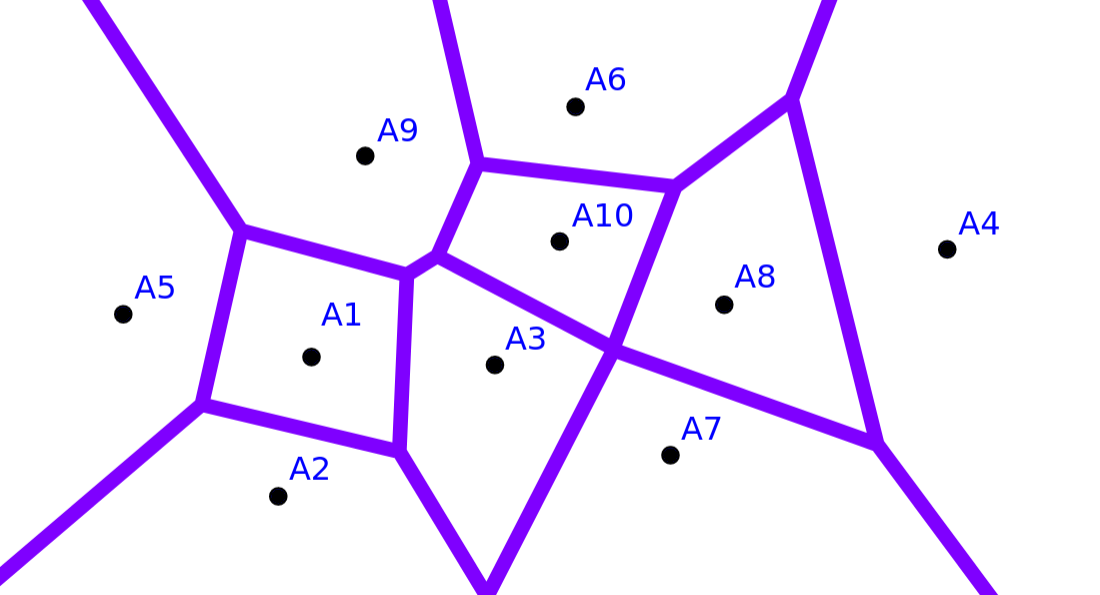
\includegraphics[width=5.5cm]{imagenes/VD.png}
  \caption{Ejemplo de un diagrama de Voronoi con diez sitios. Generado con \cite{voronoigeo}.}\label{fig:ejemploVoronoi}
\end{figure} 

 % \cite{choset2005principles}, \cite{latombe1991}, \cite{wurm2008coordinated}
\subsection{Diagrama generalizado de Voronoi}
Recordando que los sitios en un diagrama de Voronoi son puntos, se tiene un problema al querer utilizar obstáculos como sitios. El problema radica en que normalmente los obstáculos no pueden representarse como puntos en el espacio, para solucionar esto se generaliza la definición de diagrama de Voronoi para poder definirlo a partir de sitos de mayor orden, como lo son lineas, o polígonos. A esta generalización se la denomina como \emph{diagrama generalizado de Voronoi} (GVD) y los sitios de mayor orden o sitios generalizados son representados como conjuntos conexos de puntos del espacio de trabajo, siendo $\mli{GS}\subset 2^{W}$ el conjunto de todos los sitios generalizados.

% Las nuevas definiciones generalizadas son en su mayoría análogas a las originales, siendo el principal cambio la substitución de la función de distancia $d_p$ por una función de distancia generalizada $\mli{gd}_p : 2^{W} \rightarrow R$ que considera las formas de los sitios generalizados. La función $\mli{gd}_p$ se define a partir de $d_p$ como se muestra en la ecuación \ref{eq:dg}.


Las definiciones relacionadas a los GVD se basan en las definiciones planteadas para los diagramas de Voronoi pero considerando sitios generalizados en lugar de sitios puntuales. Una parte fundamental de las definiciones del GVD es la llamada función de distancia generalizada $\mli{gd}_p : 2^{W} \rightarrow R$ que considera las formas de los sitios generalizados, esta se define a partir de la distancia puntual $d_p$ como se muestra en la ecuación \ref{eq:dg}.
\begin{equation}
  \mli{gd}_p(s_i) = \min_{p'\in s_i}\{d_p(p')\} \label{eq:dg}
\end{equation}
La generalización hace necesaria la introducción del concepto de sitios base generalizados $\mli{GBS}_p$ que son los sitios mas cercanos a un punto $p$ (ecuación \ref{eq:GBS}), los cuales se utilizan para la definición de los puntos base generalizados de un punto $p$ $\mli{GBP}_p$ que son los puntos pertenecientes a los sitios de $\mli{GBS}_p$ mas cercanos a $p$ (ecuación \ref{eq:GBP}) . 
Las regiones generalizadas de Voronoi $\mli{GR}_i$ y el diagrama generalizado de Voronoi $\mli{GVD}$ son las definiciones mas similares a sus contra partes no generalizadas y se definen según se muestra en las ecuaciones \ref{eq:GR} y \ref{eq:GVD} respectivamente. 


% Notar que la definición de puntos base generalizados tiene una modificación adicional al cambio en la función de distancia, esta es que en lugar de devolver los sitios generalizados mas cercanos $\mli{GBS}_p$\ref{eq:GBS}, solo devuelve los puntos mas cercanos de estos.

\begin{equation}
  \mli{GR}_i = \{p \in W : \mli{dg}_p(s_i) \leq \mli{dg}_p(s_j), s_i,s_j\in S,s_j \neq s_i\}\label{eq:GR}
\end{equation}
\begin{equation}
  \mli{GBS}_p = \{s_i : \mli{dg}_p(s_i) \leq \mli{dg}_p(s_j), s_i,s_j\in S,s_j \neq s_i\}\label{eq:GBS}
\end{equation}
% \begin{equation}
%   \mli{GBP}_p =\{p' \in W : d_p(p') \leq d_p(p''), p' \in s_i, p'' \in s_j, s_i,s_j \in S,p' \neq p''\}
% \end{equation}
\begin{equation}
  \mli{GBP}_p =\bigcup_{s_i \in \mli{GBS}_p} \argmin_{p'\in s_i}\{d_p(p')\}\label{eq:GBP}
\end{equation}
\begin{equation}
  \mli{GVD}  = \{p \in W : |GBP_p| \geq 2\}\label{eq:GVD}
\end{equation}

En la figura \ref{fig:ejemploGVD} se muestra un ejemplo de un GVD, el espacio libre se marca con blanco, las lineas negras identifican al GVD y los polígonos negros representan obstáculos  . 

% vertices son los puntos pertenecientes al GVD, y las aristas están entre los vertices adyacentes en el espacio. Por otro lado otra forma mas compacta es que los 
% Para referirse a la segunda forma, mas compacta, de representar el GVD con un grafo se utilizara el termino grafo colapsado, y para la primera forma, el termino utilizado es grafo descolapsado. 
Los GVD suelen ser representados con un grafo en el cual los vertices son los puntos $p$ pertenecientes al GVD adyacentes a obstáculos o que cumplen con $|\mli{GBP}_p|\geq 3$, mientras que las aristas se encuentran entre los vertices que se encuentran conectados por caminos disjuntos formados por puntos pertenecientes al GVD. En la figura \ref{fig:ejemploGVDgrafo} se muestra el grafo asociado al GVD de la figura \ref{fig:ejemploGVD}, donde los círculos azules son los vertices del grafo y las lineas negras las aristas (aunque no son visibles existen aristas entre los vertices correspondientes a puntos que son tan cercanos que se solapan).

En \cite{choset2005principles} se demuestra que los GVD que utilizan obstáculos como sitios cumplen con las 3 propiedades necesarias para ser mapas de carreteras (sección \ref{subsec:mapacarr}), lo cual justifica su uso para la navegación.

% La definición de GVD puede ser con sitos base generalizados GBS en lugar de puntos base generalizado GBP:
% \begin{equation}
%   \mli{GVD}  = \{p \in W : |GBS_p| \geq 2\}\label{eq:GVD}
% \end{equation}

% Esto  necesita asumir que los obstáculos son convexos para poder entenderse porque por ejemplo si se considera las 4 paredes de una habitación como un único obstáculo eso seria un único sitio generalizado y no formaría un GVD.

% En la def que use también es necesario  porque podrían darse pequeñas imperfecciones en un espacio continuo que generen que lo que a escala macroscópica es una pared a escala microscópica sean tenga pequeñas hendiduras circulares que causen puntos pertenecientes al GVD en lugares no deseados. Esto se evita considerando obstáculos convexos. 

% La ventaja de la forma que use es que no requiere entrar en los asuntos de obstáculos convexos para un entendimiento superficial, mientras que en la otra si.

% \end{figure} 
\begin{figure}[H]
  \centering
  \subfloat[GVD]{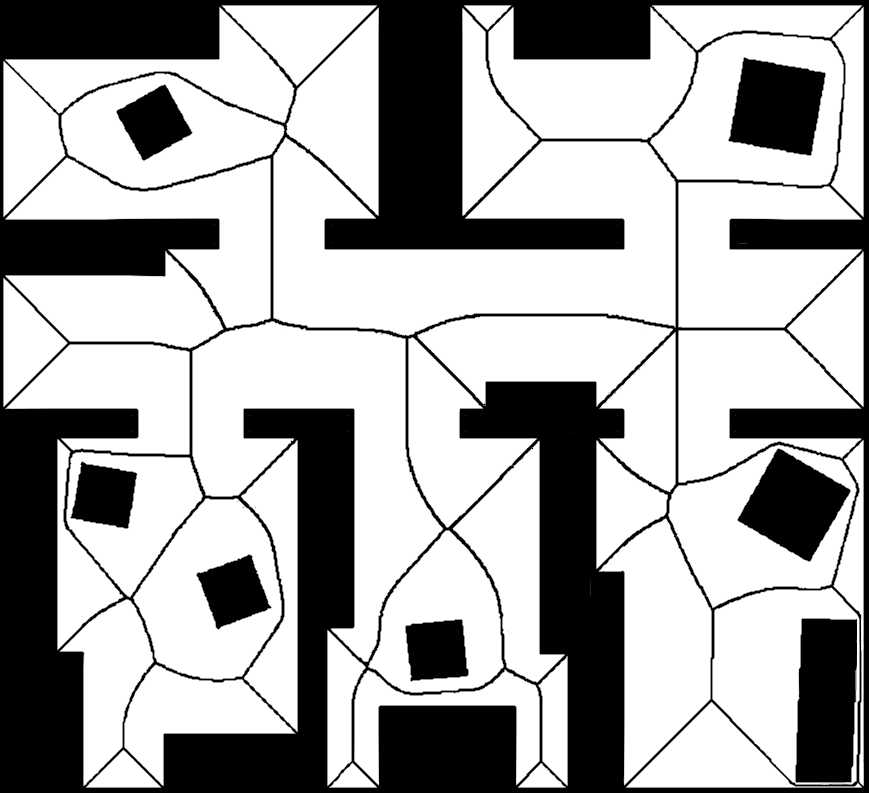
\includegraphics[clip=true, width=0.45\linewidth]{imagenes/GVD2.png}\label{fig:ejemploGVD}}
  \qquad
  \subfloat[Grafo asociado al GVD.]{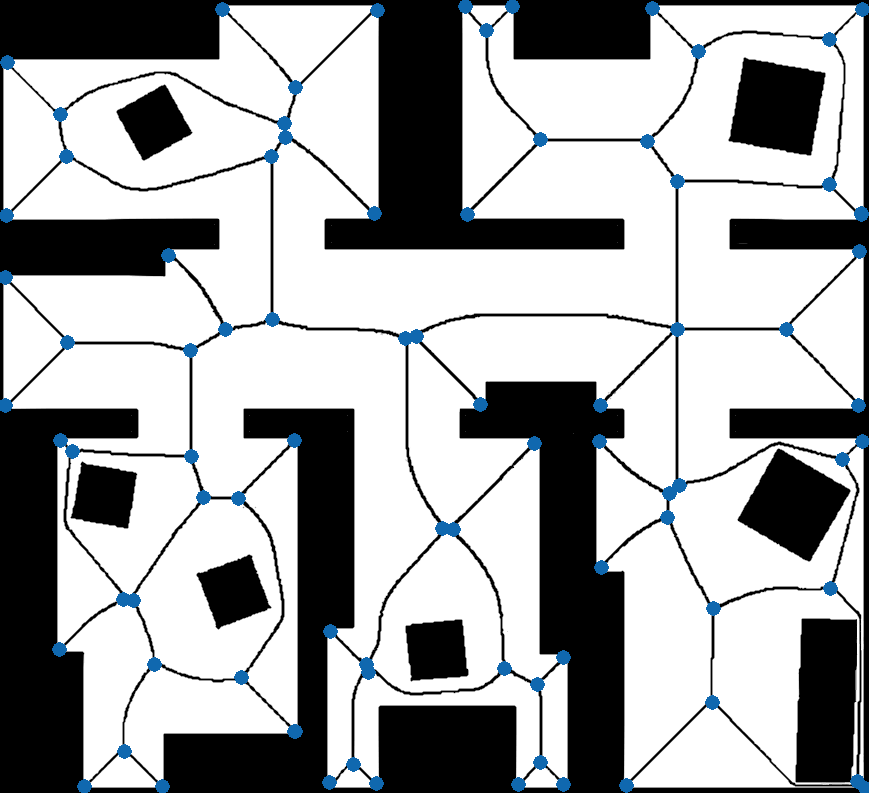
\includegraphics[clip=true, width=0.45\linewidth]{imagenes/GVDGraph.png}\label{fig:ejemploGVDgrafo}}
  \caption{Ejemplo de un diagrama generalizado de Voronoi. Extraído de \cite{Wallgrun2005}}
  \label{cleanup}
\end{figure}

\subsection{Construcción de un GVD}\label{subsec:constGVD}
Existen dos tipos principales de métodos para la construcción de un GVD los basados en sensores y los basados en grillas. En el contexto del trabajo desarrollado serán relevantes los métodos de construcción basados en grillas. 

La idea más intuitiva para generar un GVD en un espacio representado con una grilla es la de adaptar la definición original de GVD que considera espacios continuos, para que en su lugar considere espacios discretizados en celdas, y luego celda a celda, determinar según la nueva definición si estas pertenecen o no al GVD. La definición adaptada una grilla consiste en que una celda pertenece al GVD si tiene dos o mas celdas obstaculizadas a una misma distancia, siendo la distancia entre celdas la distancia entre sus centros. Sin embargo, esta técnica genera resultados erróneos al no considerar los efectos causados por la discretización. Por ejemplo, en corredores cuya discretización resulta en una cantidad par de celdas entre sus paredes, según este método ninguna celda debería pertenecer al GVD dado que ninguna  tendría una misma distancia a dos celdas obstaculizadas (paredes del corredor). Esto se considera incorrecto porque el GVD construido en un espacio discretizado debe asemejarse al GVD que se construiría en el mismo espacio si fuera continuo y  en el caso continuo los puntos del centro de un corredor siempre pertenecen al GVD. %El método de \cite{wurm2008coordinated} soluciona este tipo de problemas porque la esqueletización asegura la generación de puntos pertenecientes al GVD en las 

En \cite{wurm2008coordinated} se propone un método que logra construir un GVD evitando los problemas de discretización mencionados. El método comienza aplicando una transformación de distancia Euclidiana \cite{meijster2002general} a una mapa métrico representado con una grilla donde cada celda esta ocupada o libre , resultando en un mapa que contiene para cada celda la distancia al obstáculo mas cercano, este tipo de mapa se denomina \emph{mapa de distancia} a los obstáculos. Finalmente GVD se obtiene aplicando un algoritmo de esqueletización \cite{wan2008distance} al mapa de distancia construido. Un ejemplo de este proceso se puede ver en la figura \ref{fig:wurmGVD}.
% que consiste en erosionar las celdas mas cercanas a los obstáculos hasta llegar a las celdas mas distantes a estos siendo estas ultimas las celdas que se asignan al GVD construido. Un ejemplo de este proceso se puede ver en la figur
\begin{figure}[H]
  \centering
  \subfloat[Mapa original]{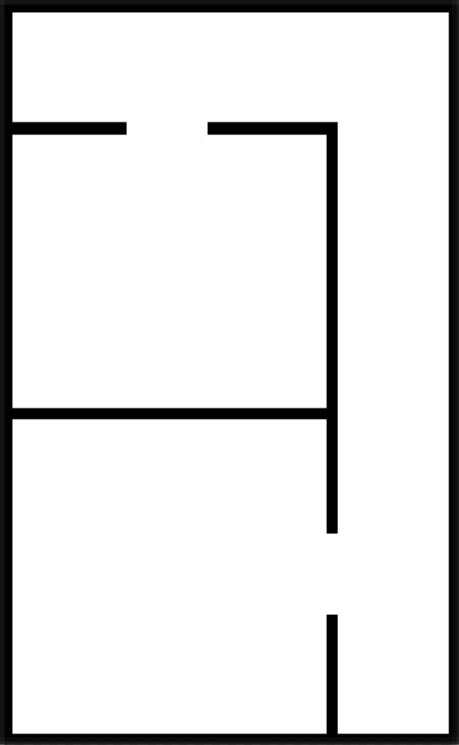
\includegraphics[clip=true, width=0.29\linewidth]{imagenes/wurmSeg/a.png}\label{fig:ejWurmA}}
  \qquad
  \subfloat[Mapa original junto a su correspondiente mapa de distancia (cuanto más oscuro es un punto, mayor es la distancia al obstáculo más cercano)]{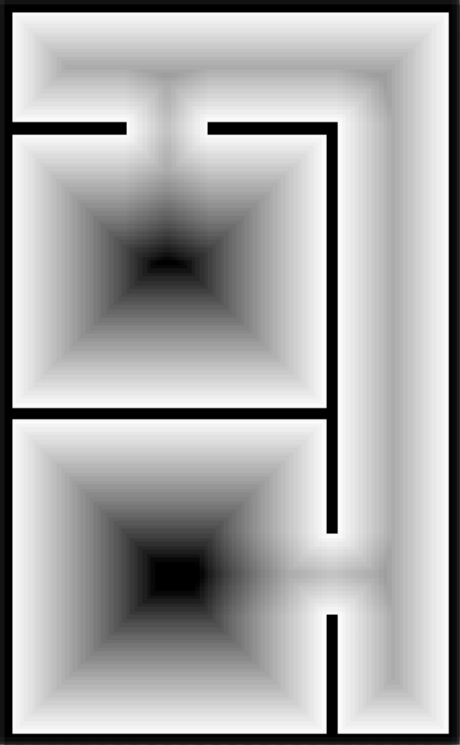
\includegraphics[clip=true, width=0.29\linewidth]{imagenes/wurmSeg/b.png}\label{fig:ejWurmB}}
  \qquad
  \subfloat[Mapa original junto al resultado de la esqueletización del mapa de distancia (lineas negras) que es a su vez el GVD construido]{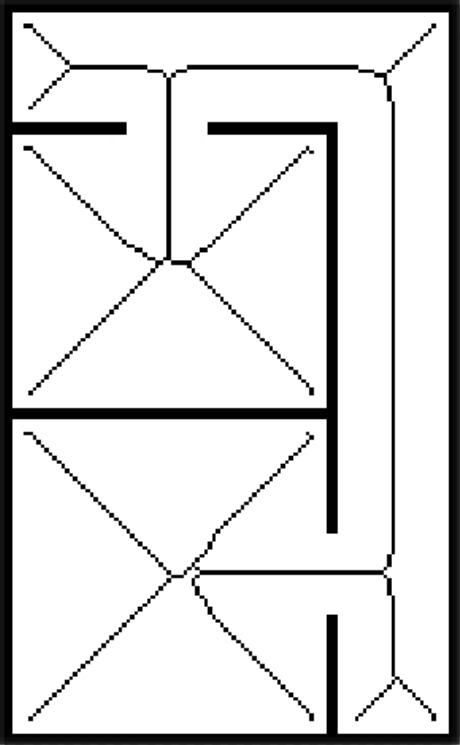
\includegraphics[clip=true, width=0.29\linewidth]{imagenes/wurmSeg/c.png}\label{fig:ejWurmC}}
  \caption{Ejemplo del método de construcción de un GVD. Extraído de \cite{wurm2008coordinated}.}\label{fig:wurmGVD}
\end{figure}
% \begin{figure}[H]
%   \begin{center}
%   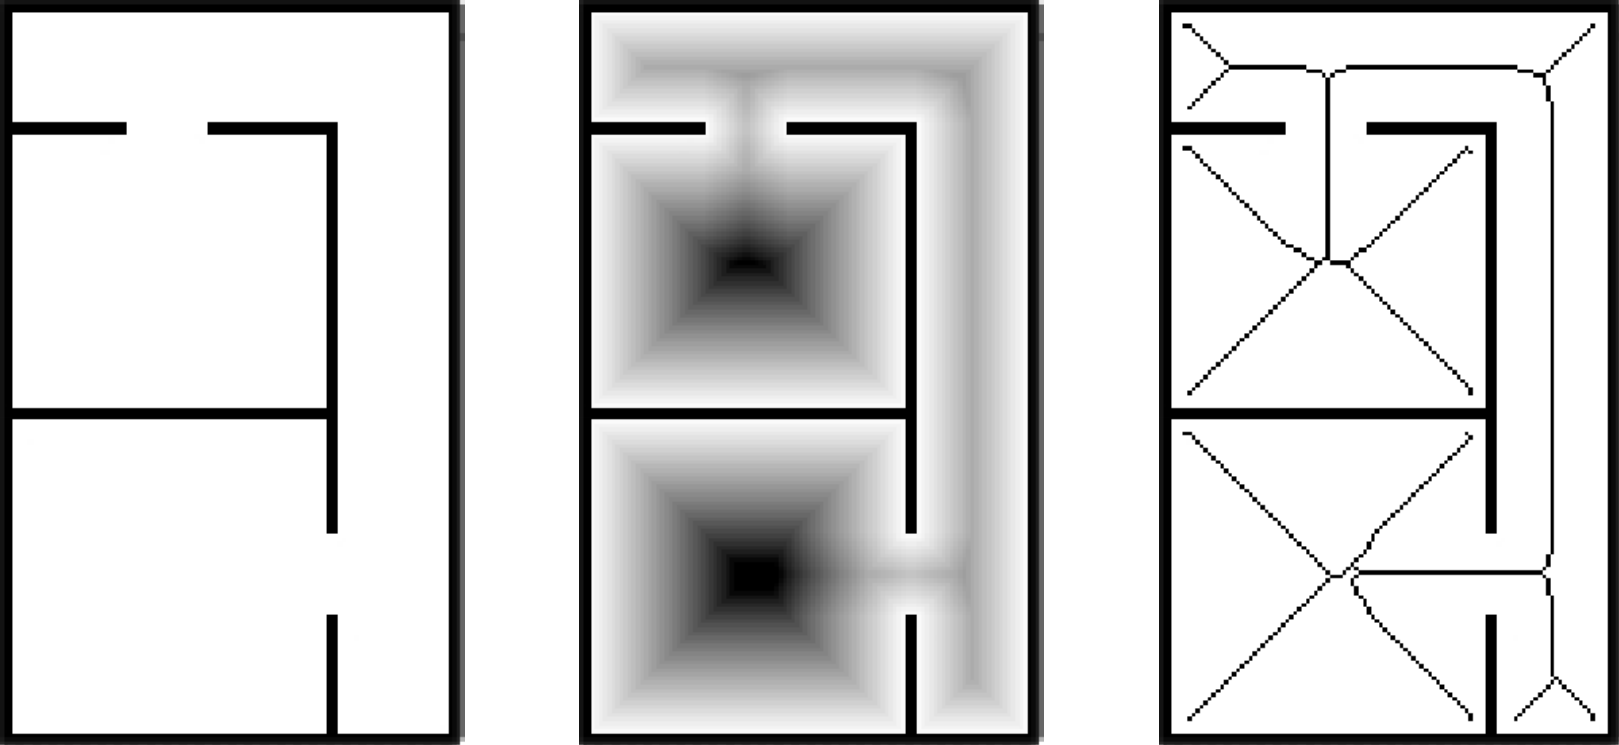
\includegraphics[width=7.5cm]{imagenes/wurmGVD.png}
%   \end{center}
%   \caption{Ejemplo del método de construcción de un GVD basado en grilla extraído de \cite{wurm2008coordinated}. A la izquierda se encuentra el mapa original, en el centro el mapa original junto a su correspondiente mapa de distancia (cuanto más oscuro es un punto, mayor es la distancia al obstáculo más cercano). A la derecha se encuentra el mapa original junto al resultado de la esqueletización del mapa de distancia (lineas negras) que es a su vez el GVD construido.}\label{fig:wurmGVD}
% \end{figure} 

% La esqueletización es usada en lugar de s
% Este método evita problemas que se pueden dar al generar un GVD discretizado a partir de la definición de pertenencia al GVD directamente adaptada a un espacio discretizado en celdas, donde una celda pertenece al GVD si tiene dos o mas celdas obstaculizadas a una misma distancia. Un ejemplo de este tipo de problemas es el que se genera en los corredores cuya discretización tiene una cantidad par de celdas entre sus paredes, en este caso si se aplica la definición de GVD a las celdas ninguna debería pertenecer al GVD dado que ninguna celda tendría una misma distancia a dos celdas obstaculizadas (paredes del corredor). Este comportamiento no es deseable ya que se debe a una discretización particular del espacio, si el tamaño de las celdas fuera otro y en lugar de ser un numero par fuera uno impar se tendría un GVD a lo largo del centro del corredor, y mas importante aun, un GVD sobre un corredor en un espacio continuo siempre genera una linea sobre el centro del corredor. %El método de \cite{wurm2008coordinated} soluciona este tipo de problemas porque la esqueletización asegura la generación de puntos pertenecientes al GVD en las 

% \begin{figure}
%   \centering
%   \subfloat[Ancho par]{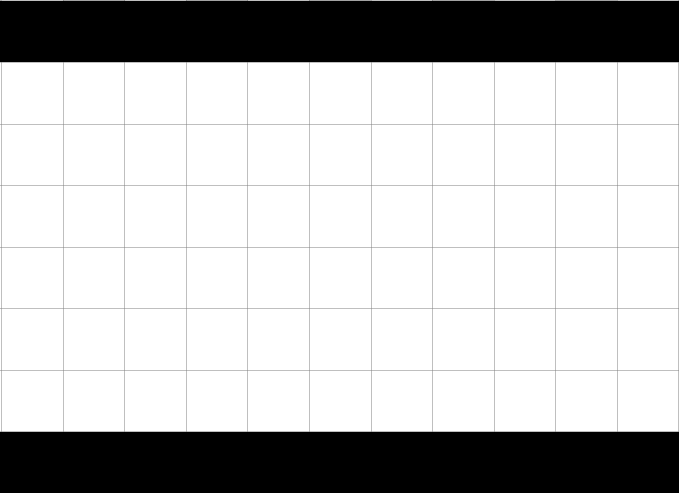
\includegraphics[clip=true, width=0.45\linewidth]{imagenes/anchopar.png}
%   \label{map:laberinto}}
%   \subfloat[Ancho impar]{\hspace{0.1\linewidth}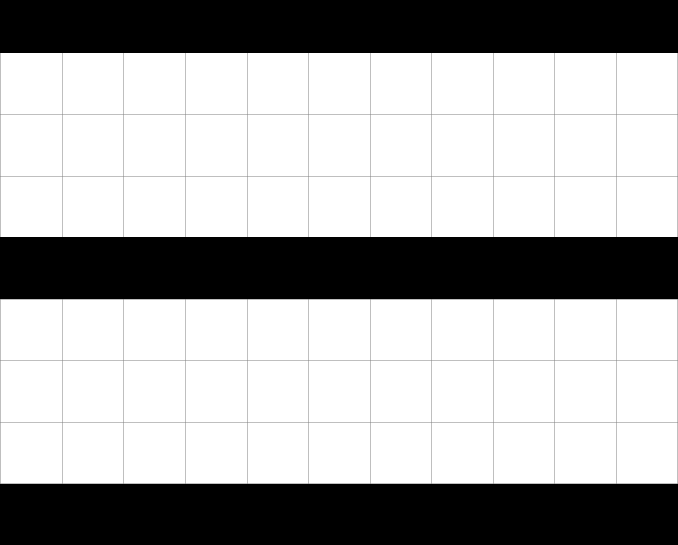
\includegraphics[clip=true, width=0.45\linewidth]{imagenes/anchoimpar.png}
%   \label{map:office}}
%   \caption{Entornos}
% \end{figure}


\subsection{Mapa topológico basado en regiones a partir de un GVD}\label{subsec:mapaTopGVD}
En \cite{Thrun1998} Thrun propone un método que permite, a partir de un mapa representado con una grilla de ocupación, segmentar el espacio en habitaciones y corredores, con el objetivo de generar un mapa topológico en el cual los segmentos serán las regiones de interés. La idea principal del algoritmo de segmentación presentado es que las entradas y salidas entre los segmentos son pasajes estrechos, y por lo tanto encontrar estos pasajes estrechos permite delimitar segmentos.

Para describir el método de segmentación necesario introducir tres nuevos conceptos asociados al GVD, el primero es el concepto de \emph{despeje} (del ingles clearance) $D : W \rightarrow R$ de un punto $p \in W$, que es igual a la distancia del punto al entorno, que si $p \in \mli{GVD}$ equivale a la distancia entre $p$ y alguno de sus puntos base generalizados $\mli{GBP}_p$ (recordar que todos están a una misma minima distancia de $p$). El segundo es el de los \emph{puntos críticos} $C \subset W_{libre}$ de un GVD, un punto es critico si este pertenece al GVD y es un mínimo local según el despeje, esta definición se formaliza en \ref{eq:crit} donde $Ady(p)$ son los vertices adyacentes a $p$ en el GVD. 
\begin{equation}
  p\ \in C \iff p \in \mli{GVD}\ \land \ D(p) < D(p')\ \forall p' \in Ady(p) \label{eq:crit}
\end{equation}
El tercer y ultimo concepto es el de \emph{linea critica}, que son las lineas que conectan a un punto critico $p \in C$ con sus puntos base $\mli{GBP}_p$.

El algoritmo comienza determinando el estado (ocupado o libre) para cada celda de la grilla de ocupación, para esto se define previamente un umbral de probabilidades, y si la probabilidad de ocupación de una celda supera dicho umbral se considera como ocupada y de lo contrario sera considerada como libre. Con la nueva grilla de estados determinados se procede a construir su  GVD. Luego se encuentran los puntos críticos asociados al GVD construido para luego obtener las lineas criticas para cada punto critico encontrado. Finalmente los segmentos serán las regiones de espacio libre delimitadas por las lineas criticas y los obstáculos. En la figura \ref{fig:ejThrunTop} se muestra un ejemplo de algunas etapas del algoritmo aplicado a un mismo entorno.

\begin{figure}[H]
  \centering
  \subfloat[GVD]{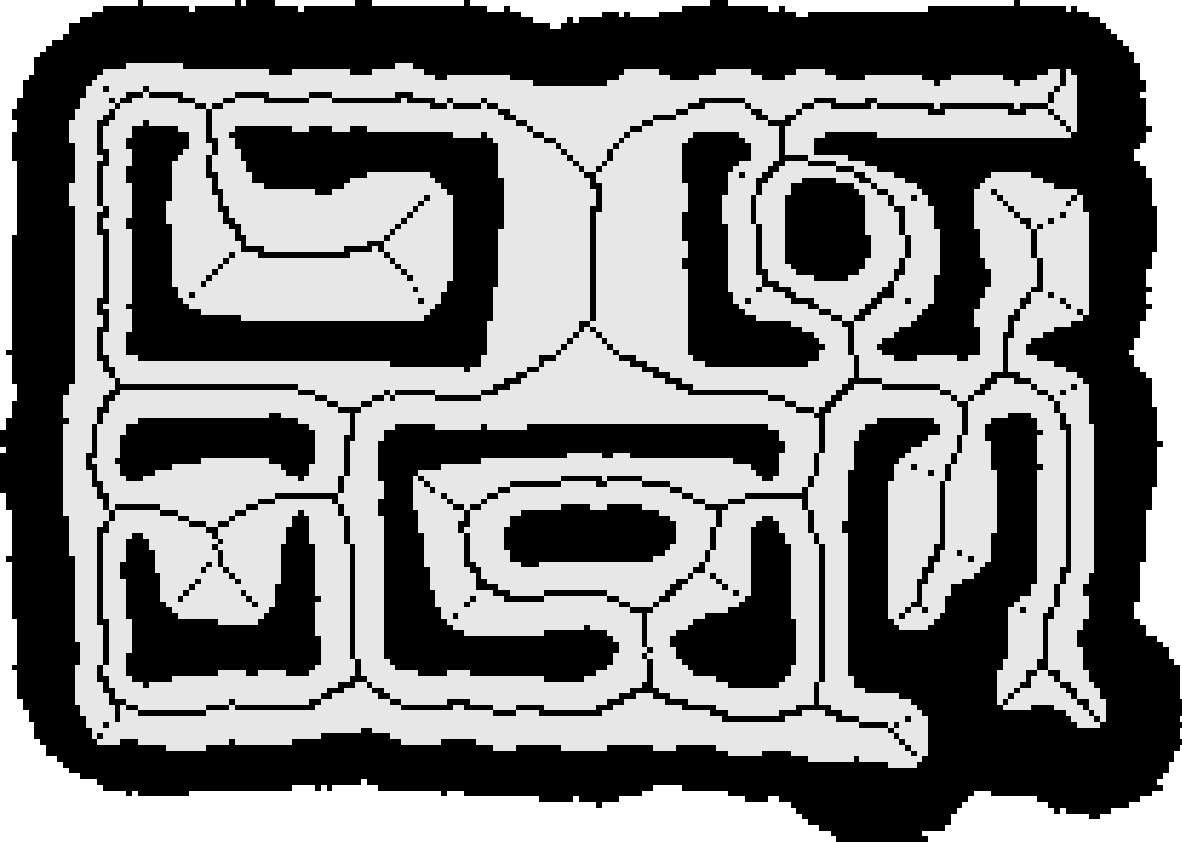
\includegraphics[clip=true, width=0.45\linewidth]{imagenes/thrunTop/a.png}\label{fig:ejThrunTopA}}
  \qquad
  \subfloat[Lineas criticas]{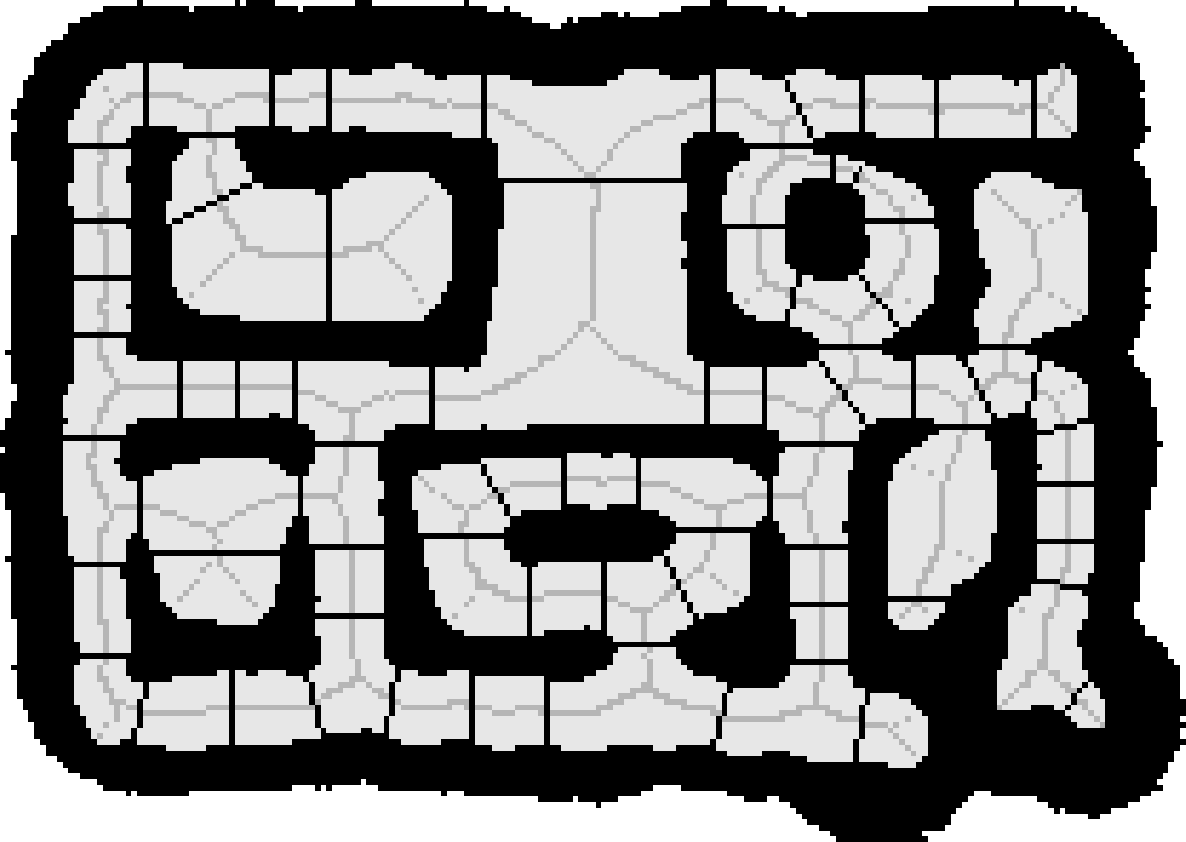
\includegraphics[clip=true, width=0.45\linewidth]{imagenes/thrunTop/b.png}\label{fig:ejThrunTopB}}
  \qquad
  \subfloat[Regiones]{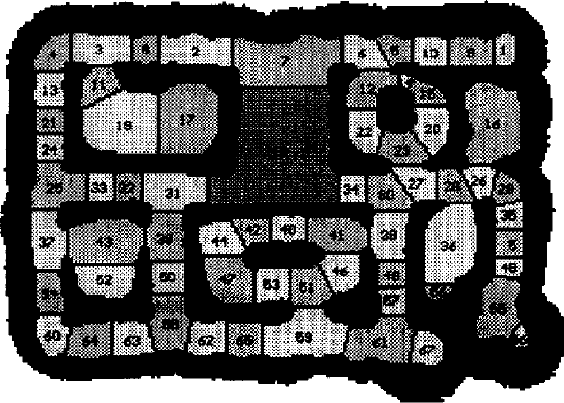
\includegraphics[clip=true, width=0.45\linewidth]{imagenes/thrunTop/c.png}\label{fig:ejThrunTopC}}
  \qquad
  \subfloat[Mapa topologico]{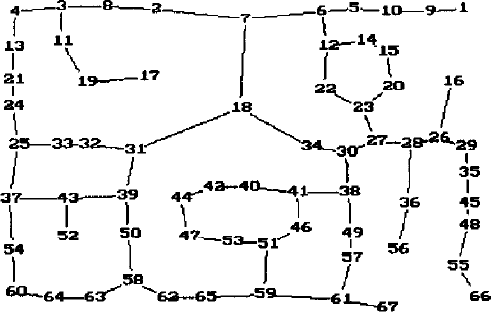
\includegraphics[clip=true, width=0.45\linewidth]{imagenes/thrunTop/d.png}\label{fig:ejThrunTopD}}
  \caption{Ejemplo del método de construcción de un mapa topológico. Extraído de \cite{Thrun1998}.}\label{fig:ejThrunTop}
\end{figure}

La idea subyacente de este algoritmo es que, por definición, los puntos críticos se encuentran presentes en el centro de todo pasaje estrecho siendo sus puntos base los extremos de dicho pasaje. Por lo tanto las lineas criticas estarán ubicadas a lo largo de cada pasaje estrecho y dada la consideración que las transiciones entre los segmentos se dan en los pasajes estrechos, las lineas criticas actúan naturalmente como limites entre cada segmento.

% TODO describir bien el algoritmo no incremental de Liu ming (capaz despues)

En \cite{wurm2008coordinated} los autores argumentan que la propuesta original de Thrun tiene el problema de generar gran cantidad de puntos críticos que no se encuentran en un pasaje entre segmentos, considerados como falsos positivos que generan una segmentación excesiva del entorno (un ejemplo de este problema se puede ver en la cantidad de segmentos generados en los corredores de la figura \ref{fig:ejThrunTopC}). Entonces, con el motivo de evitar los mencionados falsos positivos y mejorar la segmentación generada agregan condiciones adicionales a la definición de punto critico original, estas son que el vertice asociado a un punto critico en el grafo que representa GVD debe ser de grado 2 y tener un vecino de grado 3 (un vertice de intersección entre varios caminos). 

\subsection[Generación de mapas topológicos basada en contornos]{Generación de mapas topológicos basada en\\ contornos}
Existen alternativas a la generación de mapas topológicos basada en grafos generalizados de Voronoi. Una de estas es la generación de mapas topológicos basada en contornos presentada en \cite{Fermin-Leon2017}. Esta se basa en representar a la grilla de ocupación como una imagen, extraer sus contornos los cuales se representan como polígonos y a partir de su convexidad se segmentar el espacio, obteniendo así un mapa topológico.

\subsection{Criterios de calidad de un mapa topológico basado en regiones}
Según \cite{Liu2015} un mapa topológico basado en regiones se considera útil si representa la estructura del entorno de manera correcta y eficiente. Para ello, consideran dos criterios principales, la calidad asociada a cada region y la topología la segmentación. Los criterios propuestos se basan principalmente en intuiciones geométricas. 

\subsubsection{Calidad de una region}
Los autores determinan que existen dos aspectos que intervienen en la calidad de una region, la convexidad $c_i$ y la compacidad $s_i$, específicamente, definiendo la calidad de una region como $q_i = c_i - s_i$. Adicionalmente se menciona que tanto $c_i$ como $s_i$ pueden ser multiplicados por pesos en el calculo de $q_i$ para  para hacer énfasis en una u otra característica.

\paragraph{Convexidad}
% Convexity: A polygon is considered convex if for any pair of points inside the polygon, every point on the straight line segment that joins them is also inside the polygon.
Esta se puede representar como el cociente entre el area de la region y el area de su envolvente convexa. La envolvente convexa de una region se define como el polígono convexo de menor area que contiene a la region. Un polígono convexo cumple que para cualquier par de puntos que pertenecen a la frontera del polígono, el segmento de recta que los conecta estará contenido en dicho polígono. Entonces sea $A_i$ el area de la region $R_i$ y $H_i$ el area de su envolvente convexa, la convexidad para esta region sera:
\begin{equation}
  c_i=\frac{A_i}{H_i}
\end{equation}
Se cumple que $A_i \leq H_i$ siendo iguales cuando la region es convexa, por lo tanto $c_i$ sera igual a uno cuando la region es convexa, y su valor disminuirá entre más difiera el area de la region con la de su componente convexa. En la figura \ref{fig:ejemplConvexidad} se muestra a modo de ejemplo el valor de convexidad $c$ asociado a dos regiones con distinta convexidad.
\begin{figure}[H]
  \centering
  \subfloat[c=0.88]{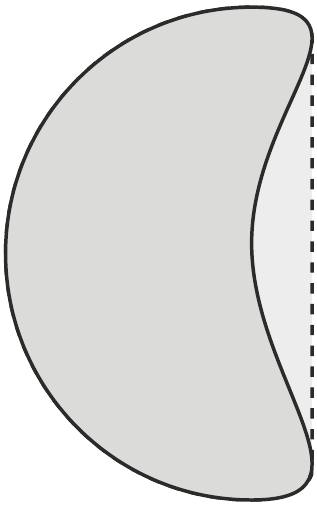
\includegraphics[clip=true, height=0.25\linewidth]{imagenes/liuConv/a.png}}
  \hspace{2cm}
  \qquad
  \subfloat[c=0.56]{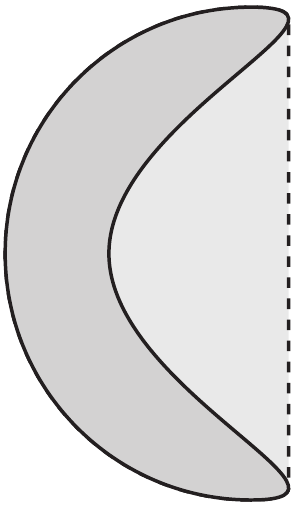
\includegraphics[clip=true, height=0.25\linewidth]{imagenes/liuConv/b.png}}
  \caption{Dos regiones con su valor de convexidad asociado, las lineas solidas delimitan la region y las lineas punteadas delimitan su envolvente convexa. Extraído de \cite{Liu2015}.}\label{fig:ejemplConvexidad}
\end{figure}

\paragraph{Compacidad}
% Cuanto mas cercanos son los puntos que componen una region a su centro mas compacta sera la region.
La compacidad de una region mide la distribución una region con respecto a su centro de masa. La compacidad $s_i$ de una region $R_i$ se calcula a partir de una discretization de dicha region en celdas de dimensiones y peso uniforme, llamadas elementos de masa. La ecuación \ref{ec:compacidad} define la compacidad $s_i$ para un region $R_i$, donde $x_j$ e $y_j$ son las coordenadas x e y de los elementos de masa de $R_i$, $M_i$ es igual a la cantidad de dichos elementos de masa y $x_0$ e $y_0$ son las coordenadas del centro de gravedad de $R_i$.
\begin{equation}
  s_i=\frac{1}{M_iA_i}\sum_j \frac{(x_j-x_0)^2 + (y_j-y_0)^2}{A_i} \label{ec:compacidad}
\end{equation}
Notar que cuanto mas compacta sea una region menor sera su valor $s_i$ (si se entiende por region compacta una region en la cual sus puntos interiores son cercanos al centro de masa).

\subsubsection{Calidad de segmentación}
Para determinar la calidad general de la segmentación, sera necesaria, ademas de la calidad de cada region, la calidad de las características globales de la segmentación. Para lograr determinar dichas características se definen varios indicadores que se mencionarán a continuación.

\paragraph{Cobertura}
En el caso ideal cada punto del entorno esta asociado a una region en el mapa topológico, pero por diversas razones este puede no ser el caso. Dado esto se define la cobertura $C$ de una segmentación como el cociente del area representada por el mapa topológico y el area del mapa:
\begin{equation}
C=\frac{\sum^N_{i=1} A_i}{A_m}
\end{equation}
Donde $A_m$ es el area total del mapa y $N$ es el numero de regiones.

\paragraph{Validez}
La validez $V$ de una segmentación se define como el cociente entre el numero de regiones validas y el numero total de todas las regiones:
\begin{equation}
  V=\frac{\#regiones\ validas}{\#total\ de\ regiones}
\end{equation}
Se considera que una region valida debe ser accesible por los robots utilizados. Teniendo esto en cuenta una region será valida si cubre un area mayor a $A_{min}$ y tiene al menos una entrada de ancho mínimo $l_{min}$, siendo los valores $l_{min}$ y $A_{min}$ definidos a partir las dimensiones de los robots utilizados.

\paragraph{Simplicidad}
Una de las ventajas principales de los mapas topológicos es su simplicidad, que permite ayudar a una navegación y planificación eficiente. Los autores consideran que es de utilidad penalizar a los mapas topológicos que tengan una cantidad elevada de regiones, considerando dicha cantidad como un indicador de complejidad. 

La simplicidad $S$ de una segmentación se define en la ecuación \ref{ec:simp} donde $\hat{N}$ es el numero esperado de regiones y $\phi$ refleja el impacto que tiene la diferencia entre el numero de regiones esperado y el obtenido. $\hat{N}$ y $\phi$ son parámetros a definir dependiendo de la aplicación.

\begin{equation}
  S=e^{-\frac{|N-\hat{N}|}{\phi}} \label{ec:simp}
\end{equation}


\subsubsection{Calidad general}
Finalmente, evaluar la calidad general $Q$ de una segmentación, se reduce a combinar la calidad cada región y los indicadores de calidad de la segmentación, según la siguiente ecuación:
\begin{equation}
Q=\frac{CV}{N}\sum^N_{i=1}{q_i+\lambda S}
\end{equation}

Donde $\lambda$ es un peso que determinara la importancia de la simplicidad de la segmentación en cálculo calidad general de la segmentación.

% \subsubsection{Evaluación humana}
% Otra criterio de evaluación es el utilizado en \cite{Fermin-Leon2017} el cual compara la segmentación a evaluar $R_{seg}$ contra segmentaciones realizadas por humanos $R_{human}$. La comparación consiste en para cada pixel comprobar si este esta asignado a una misma region en ambas segmentaciones, lo cual se considera como un verdadero positivo $vp$, los falsos positivos $fp$ son los pixeles que están en la segmentación a evaluar pero no en la humana, o no, que se considera  

\subsection{Eficiencia en la construcción del GVD y de mapas topológicos a partir de un GVD}
% A lo largo de la exploración el mapa construido recibirá, de forma frecuente, actualizaciones que solo modifican una pequeña porción del mismo. Dado esto, por motivos de eficiencia, se busca que los algoritmos que utilizan al mapa como una entrada eviten recomputarse completamente en cada actualización y que en su lugar actualicen el ultimo resultado obtenido para que sea consistente con la ultima version del mapa.

% Los algoritmos que requieren recomputarse completamente al cambiar parte de la entrada son conocidos como \emph{algoritmos no incrementales}, por otro lado los algoritmos que actualizan la salida anterior a partir de los cambios experimentados desde la ultima entrada son llamados \emph{algoritmos incrementales}.

% Los algoritmos de generación de GVD, y de segmentación a partir de un GVD descritos anteriormente son no incrementales, por lo tanto dado el problema de eficiencia que esto implica es de interés describir variantes incrementales para los mismos.

A lo largo de la exploración el mapa construido recibe actualizaciones de forma frecuente que solo modifican una pequeña porción del mismo. Esto causa que los datos que tienen que ser consistentes con el mapa también deban actualizarse de forma frecuente. Dado esto, por motivos de eficiencia, se busca que los algoritmos que deben ejecutarse para mantener la consistencia de los datos con el mapa, eviten descartar el resultado anterior y recomputarse completamente en cada actualización, sino que en su lugar modifiquen el ultimo resultado para que este sea consistente con la ultima version del mapa. 

La idea se basa en que, como se mencionó anteriormente, las actualizaciones son frecuentes pero también pequeñas y por lo tanto luego de una actualización gran parte del mapa se mantiene igual. Esto usualmente implica que gran parte del resultado anterior continua siendo valido luego de la actualización, solo siendo necesario modificar una pequeña porción del mismo para que este vuelva a ser consistente, lo cual suele ser órdenes de magnitud menos costoso que la alternativa de calcular todo desde cero. 
 % hecho de que las actualizaciones solo modificaron una  que e 

% Los algoritmos que requieren recomputarse completamente al cambiar parte de la entrada son conocidos como \emph{algoritmos no incrementales}, por otro lado los algoritmos que actualizan la salida anterior a partir de los cambios experimentados desde la ultima entrada son llamados \emph{algoritmos incrementales}.
Los algoritmos que actualizan el resultado anterior a partir de los cambios experimentados son llamados \emph{algoritmos incrementales}, en consecuencia los que algoritmos que al cambiar parte de la entrada descartan el ultimo resultado y recomputando el nuevo resultado desde cero se denominan como \emph{algoritmos no incrementales}.

En las secciones \ref{subsec:constGVD} y \ref{subsec:mapaTopGVD} los algoritmos presentados son no incrementales, dado el problema de eficiencia que esto implica son de interés sus variantes incrementales que se explicarán a continuación.
% Los algoritmos de generación de GVD, y de segmentación a partir de un GVD presentados anteriormente no son incrementales, dado el problema de eficiencia que esto implica son de interés las variantes incrementales que se explicarán a continuación.

% , y por lo tanto su uso resulta ineficiente, por esto fueron desarrolladas variantes incrementales para los mismos.
\subsubsection{Construcción incremental del GVD}
% El algoritmo incremental para la construcción de un GVD que se presentara en esta sección es conocido como \emph{brushfire dinámico}, formulado originalmente por Karla \textit{et al.} en \cite{kalra2009incremental}. Este algoritmo se basa en el algoritmo no incremental \emph{brushfire}

El algoritmo \emph{brushfire} permite determinar el mapa de distancia a los obstáculos, asociado a una grilla donde cada celda tiene asociado un estado libre u ocupado. Este algoritmo se puede ver como una variante al conocido algoritmo de Dijkstra que permite varias fuentes y no tiene destino, donde las fuentes son los obstáculos y la distancia calculada es la minima distancia hacia un obstáculo. Se comienza inicializando las distancias de las celdas libres con $\infty$ y las obstaculizadas con $0$. Adicionalmente, las celdas obstaculizadas se insertan en una cola de prioridad que prioriza las celdas de menor distancia. Luego hasta que las cola de prioridad este vacía se remueve la celda mas prioritaria $c$ y para cada celda $c'$ adyacente a $c$ se computa una distancia tentativa $dt_{c'}$ según la ecuación \ref{ec:dtBrushFire} que remplaza la distancia actual $d_{c'}$ de la celda $c'$ si $dt_{c'}<d_{c'}$. De reemplazarse $d_{c'}$ se inserta a $c'$ en la cola de prioridad. 

\begin{equation}\label{ec:dtBrushFire}
  dt_{c'} = d_c+||c'-c||_2
\end{equation}

Una vez que la cola de prioridad queda vacía, el valor de distancia de las celdas converge al valor de la minima distancia hacia un obstáculo. 

El nombre de este algoritmo proviene de como este determina las distancias comenzando desde cada obstáculo y extendiéndose desde las celdas mas cercanas a las mas lejanas asemejándose a un incendio de maleza (traducido al ingles como brushfire). Adicionalmente el algoritmo también puede interpretarse como ondas que parten desde cada obstáculo, y a medida de que avanzan le asignan la distancia recorrida a las celdas que atraviesan. Un ejemplo de ejecución se muestra en la figura \ref{fig:wavesBrush}.  
% a cada celda por la que pasan mientras avanzan

\begin{figure}[H]
  \center
  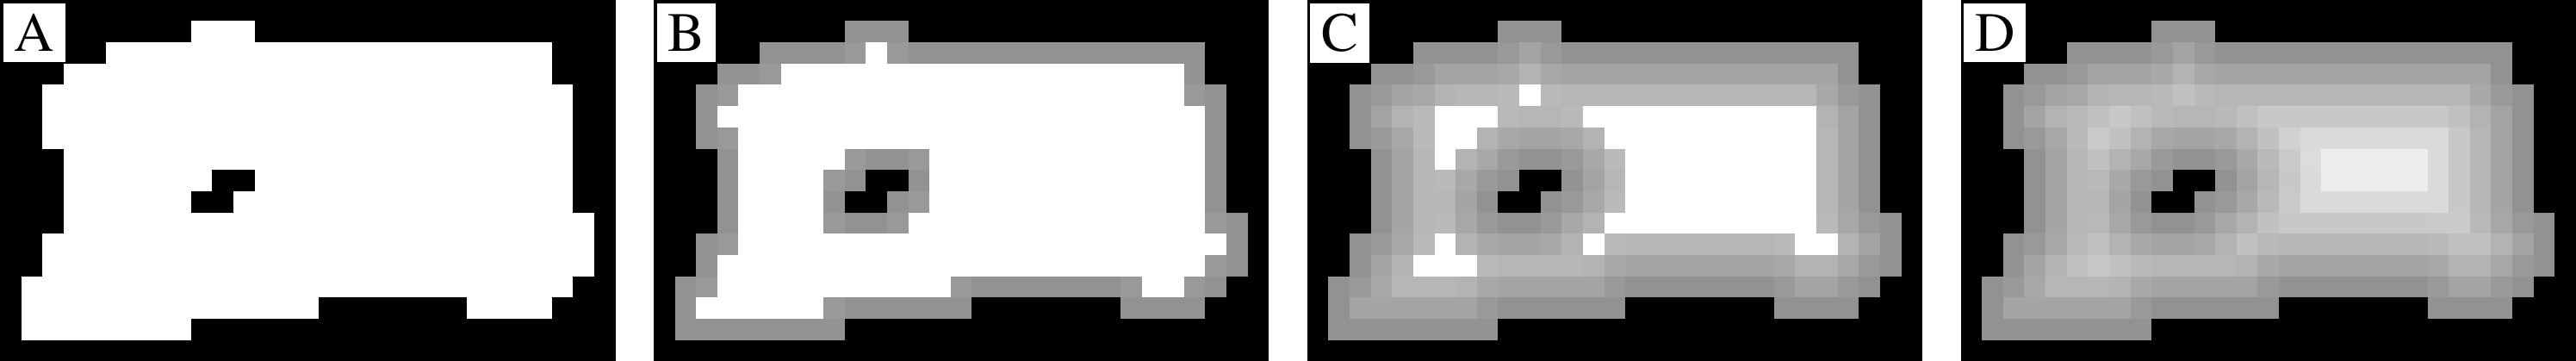
\includegraphics[width=1\linewidth]{imagenes/wavesBrush.png}
  \caption{Ejemplo de brushfire. (A) Los valores de distancia se inicializan con 0 (negro) para celdas ocupadas e infinito (blanco) para celdas vacías. (B) y (C) Las celdas ocupadas generan ondas que asignan distancias crecientes a medida que se propagan, indicadas por el aumento de brillo de las celdas. (D) Las ondas se detienen al no poderse reducir más valores de distancia. Una vez que se han detenido todas las ondas, se obtiene el mapa de distancia completo. Extraído de \cite{Lau2013}.}\label{fig:wavesBrush}
\end{figure} 

En \ref{subsec:constGVD} se muestra un método de construcción que requiere primero encontrar un mapa de distancia y luego aplicar un algoritmo de esqueletización, pero brushfire puede ser adaptado para construir el GVD sin el paso intermedio de esqueletización. La idea se basa en asignar identificadores a cada conjunto conexo de celdas obstaculizadas y luego según la interpretación de brushfire como ondas, las ondas provenientes de celdas obstaculizadas con identificadores distintos colisionan en las celdas que deben pertenecer al GVD. 

El algoritmo de brushfire descrito hasta el momento no es incremental, pero en \cite{kalra2009incremental} Kalra \textit{et al.} presentan una variante nombrada \emph{brushfire dinámico} que si lo es.

Como se comento anteriormente, los algoritmos incrementales fundamentalmente consisten en tomar como entrada los cambios ocurridos desde la ultima ejecución, y a partir de estos modificar solo las porciones del ultimo resultado necesarias para que vuelva a ser consistente. En este caso los cambios ocurridos corresponden a un conjunto de celdas en las que su estado pasa de ser obstaculizado a ser libre o viceversa. 

Partiendo de un mapa de distancias parcialmente correcto brushfire dinámico propaga los cambios ocurridos en forma de ondas. Las celdas $o$ que pasan a estar obstaculizadas emiten una onda \say{consistente} que establece la distancia $dt_c$ recorrida por la onda a la nueva distancia $d_c$ asociada a la celda $c$ si $dt_{c}<d_{c}$, si la distancia se modifica se establece a $o$ como el obstáculo a minima distancia de $c$. En el caso de las celdas $l$ que pasan a estar libres emanan una onda \say{inconsistente} que reinicia a $\infty$ (invalida) las distancias $d_c$ de las celdas $c$ que tienen a $l$ como obstáculo a minima distancia, esta onda se expande hasta llegar a una celda $c'$ que tiene obstáculo valido a minima distancia, al suceder esto desde $c'$ se resume la onda \say{consciente} que causo su valor de distancia actual de forma de restablecer la distancia de las celdas reiniciadas. En la figura \ref{fig:wavesBrushDyn} se muestra gráficamente el funcionamiento de brushfire dinámico.

\begin{figure}[H]
  \center
  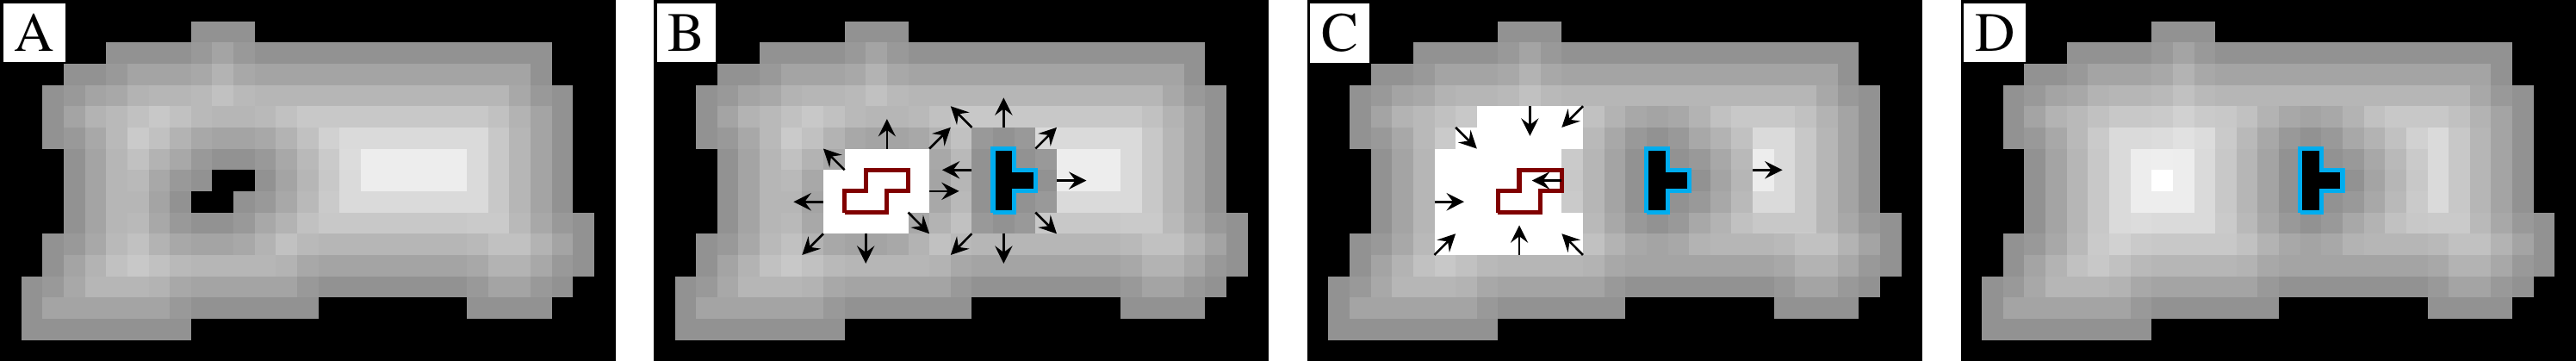
\includegraphics[width=1\linewidth]{imagenes/wavesBrushDinClean.png}
  \caption{Ejemplo de brushfire dinámico. (A) Ultimo mapa de distancias calculado. (B) Un obstáculo es eliminado (contorno rojo) lo cual causa ondas inconsistentes que comienza a reiniciar los valores de distancia inválidos, a su vez un obstáculo es insertado (contorno azul) y generando ondas consistentes que propagan las nuevas distancias. (C) Cuando las ondas inconsistentes chocan contra celdas con un obstáculo más cercano válido estas se detienen y en ese mismo lugar inicia una onda consistente para restaurar los valores de distancia reiniciados. (D) Después que todas las ondas se detienen, la actualización se completa. Extraído de \cite{Lau2013}.}\label{fig:wavesBrushDyn}
\end{figure} 

Con esto se tiene una definición de brushfire dinámico que calcula un mapa de distancia. De forma análoga a lo realizado en brushfire, brushfire dinámico se puede adaptar para lograr construir un GVD, pero en este caso de forma incremental. Las ondas consistentes causan la pertenecía al GVD de las celdas en donde estas se detienen y de las celdas que causaron que se detengan. Por otro lado las ondas inconsistentes remueven del GVD a todas las celdas cuya pertenencia al GVD involucra a celdas previamente obstaculizadas que pasaron a ser libres.

\begin{figure}[H]
  \center
  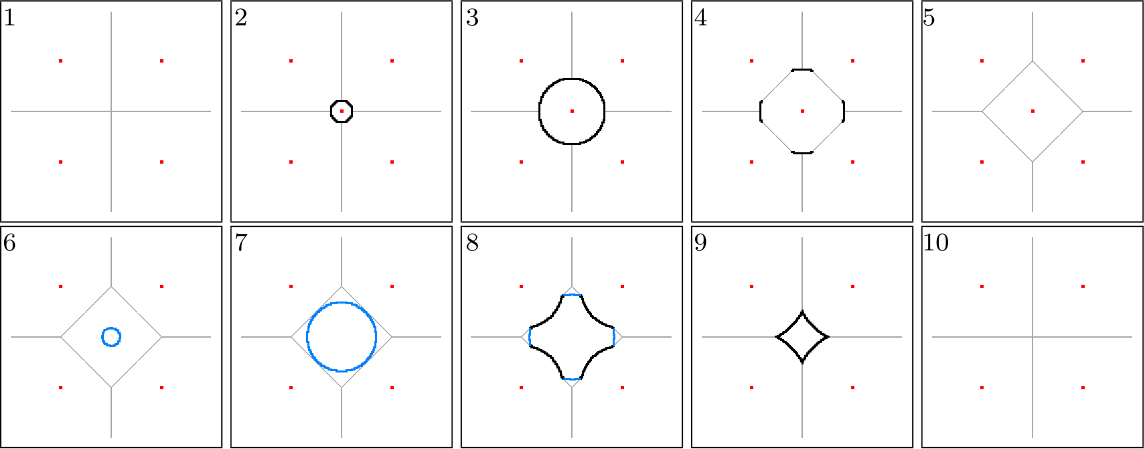
\includegraphics[width=1\linewidth]{imagenes/wavesKalra.png}
  \caption{Una secuencia que ejemplifica las olas generadas cuando se agregan obstáculos (1-5) y se eliminan obstáculos (6-10). (1-5) Se agrega nueva celda obstaculizada en el centro del entorno (en rojo) lo cual produce una ola consistente (en negro) que al detenerse genera celdas pertenecientes al GVD (en gris). (6-10) La celda central se elimina produciéndose una ola inconsistente (en azul) que remueve las celdas del GVD que involucran a la celda obstaculizada que paso a ser libre mientras que al al llegar a cedas con una distancia minima generar olas inconsistentes (en negro) que reparan el GVD. Extraído de \cite{kalra2009incremental}.}\label{fig:ejWavesIncKarlra}
\end{figure} 


De esta forma se logra la construcción incremental de un GVD. Sin embargo en \cite{Lau2013} Lau \textit{et al.} destacan algunas problemáticas de brushfire dinámico, principalmente, que genera un GVD con lineas de dos celdas de ancho y que por basar la generación en los conjuntos conexos de obstáculos no genera celdas pertenecientes al GVD dentro de los conjuntos conexos de obstáculos que a su vez son cóncavos. Estos problemas se pueden ver en a la izquierda de la figura \ref{fig:lauPalo}.
% Nuestro enfoque genera líneas de Voronoi delgadas, de modo que diferentes caminos en el GVD corresponden a rutas topológicamente diferentes.
\begin{figure}[H]
  \center
  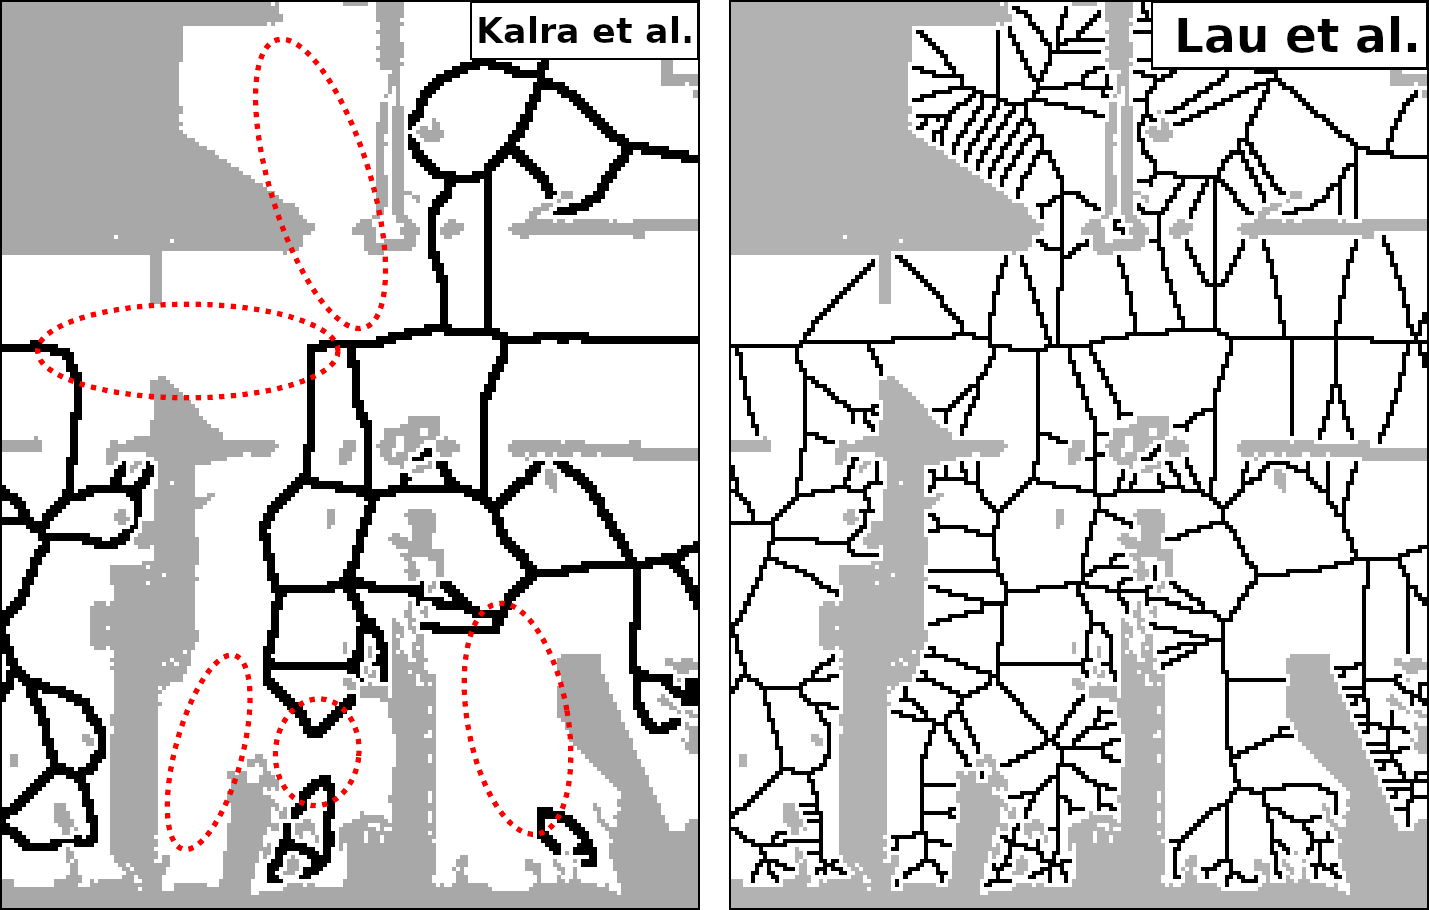
\includegraphics[width=0.75\linewidth]{imagenes/lauPalo.png}
  \caption{GVD calculado con el algoritmo de brushfire dinámico original a la izquierda y el calculado por el brushfire dinámico modificado de Lau \textit{et al.} a la derecha. Las elipses marcan las líneas de Voronoi que faltan.  Extraído de \cite{Lau2013}.}\label{fig:lauPalo}
\end{figure} 

% Sin
% En el caso anterior la onda solo puede reducir la distancia $d_{c'}$ de una celda $c'$, esta es la principal diferencia con las ondas que provienen de una celda que pasa de estar ocupada a estar libre, en este caso se tendra una onda que aumentara la distancia  


% Según la interpretación de brushfire como ondas se tiene que las celdas que pertenecen al GVD serán las que se 

% En \cite{kalra2009incremental} Kalra \textit{et al.} proponen un algoritmo que se basa en el algoritmo no incremental llamado brushfire \cite{choset2005principles} cuyo propósito es computar el mapa de distancia,  La idea de este algoritmo
% El principal problema con este acercamiento es que el GVD se construye basa en determinar obstáculos independientes para luego calcular el GVD. Esto es un problema porque no es claro en como pasar de celdas obstaculizadas a obstáculos que están compuestos por estas (buscar mas problemas, ineficiencia?, nuestro código no lo soportaba de antes).  El siguiente artículo propone una solución que evita esta necesidad y solo basta con tener un grilla de ocupación.


\subsubsection{Construcción incremental de mapas topológicos a partir de un GVD}
\cite{Liu2015}

% Articulo del cual obtuvimos varias las características de nuestra implementación incremental

% como entrada eviten re 
%  computar los cambios que se deben realizar a dicho resultado para que este corresponda al resultado del mapa actualizado.  


% computarse completamente con cada cambio y que en su 

% Los algoritmos presentados hasta el momento son todos no incrementales, en tanto si el mapa sobre el cual se construyen cambia, e

% en esta sección se trataría sobre las diferencias entre incremental y no incremental, mencionar lo que se gana en performance y que implica una dificultad mayor, y después comentar bien como es la:

% generación de GVD incremental

% segmentación incremental (mencionar también que la contorno también tiene variante incremental)

% Luego comentar nuevamente las técnicas de remoción de falsos positivos de Wurm y la diferencia entre utilizarlas y no (usar de ejemplo resultados de Liu ming) esto para decir que una de las cosas que se hace en el desarrollo es generar un algoritmo que hace esto

\subsection{Coordinación en la exploración multirobot}
Como fue mencionado en la sección \ref{subsec:expmutirob}, la coordinación es un aspecto critico en problema de exploración multirobot, por lo tanto a lo largo del tiempo fuero desarrolladas varias propuestas para una exploración multirobot coordinación. A continuación se describen técnicas de coordinación que consisten en primero segmentar el espacio, asignar segmentos a los robots, para finalmente establecer los objetivos de exploración de robots teniendo en cuenta el segmento asignado y el segmento al que pertenece el objetivo. Las propuestas se dividen en las que segmentan el espacio considerando la topología del mismo los que segmentan según criterios no topológicos.
 % para la coordinación de una flota robótica durante la tarea de exploración de un entorno desconocido
% para la exploración multi-robot 
\subsubsection{Coordinación a partir de mapas topológicos}
% En \cite{wurm2008coordinated} se describe y analiza un enfoque de coordinación que se basa en la distribución eficiente de los robots durante la exploración, teniendo en cuenta la estructura del entorno a partir del uso de mapas topológicos.

En \cite{wurm2008coordinated} se describe y analiza un enfoque de coordinación que tiene en cuenta la estructura del entorno a partir del uso de mapas topológicos. La estrategia de coordinación consiste en la distribución uniforme de los robots sobre las habitaciones y corredores (segmentos), que componen a un entorno estructurado. Esto se basa, en primera instancia, en que asignar más de un robot a un mismo segmento en muchos casos puede ser una desventaja ya que este podría ser demasiado pequeño para que un segundo robot acelere su exploración aunque exista más de un objetivo de exploración en el mismo, e incluso al terminar la exploración de un segmento los robots pueden bloquearse entre sí mientras intentan abandonarlo. Por otro lado las tareas de exploración de segmentos diferentes suelen en su mayor parte ser independientes entre si. Considerando esto, distribuir los robots sobre los segmentos a explorar debería lograr una reducción del trabajo redundante y de las interferencias entre los mismos, llevando a una reducción del tiempo de exploración.

Implementar esta técnica de coordinación requiere la construcción de un mapa topológico ya que con este se obtiene la información sobre los segmentos del entorno. Para la construcción de el mapa topológico los autores utilizan la técnica descrita en \ref{subsec:mapaTopGVD}, que consiste en la construcción del mapa topológico a partir de un GVD y el método de construcción del GVD utilizado es el explicado en \ref{subsec:constGVD}.

La idea es que al asignar un robot a un segmento este deberá completar los objetivos de exploración que estén dentro de dicho segmento, siendo los objetivos, como es usual, las fronteras entre las partes desconocidas y conocidas del mapa. 

% Los entornos interiores son en general estructurados, por ejemplo, los edificios generalmente se dividen en habitaciones a las que se puede llegar por pasillos.
Para asignar los objetivos a los robots primero estos son asignados a los segmentos a explorar, de forma de maximizar la distribución de los robots sobre los segmentos, por ejemplo evitando asignar mas de un robot por segmento si la cantidad de segmentos a explorar es mayor que la cantidad de robots. Dicha maximización se obtiene cuando los robots están distribuidos de forma uniforme en los segmentos, cosa que se obtiene si se cumple lo planteado en la ecuación \ref{ec:uniform} donde $S$ es el conjunto de todos los segmentos del mapa topológico, y $\#Robots : S \rightarrow N$ es una función que dado un segmento devuelve el numero de robots asignados al mismo. 

\begin{equation}\label{ec:uniform}
  \forall s,s' \in S, |\#Robots(s) - \#Robots(s')| <= 1
\end{equation}

Para resolver la asignación se propone el uso del método húngaro\cite{kuhn1955hungarian} de una forma particular que permite cumplir con la restricción \ref{ec:uniform}. Para ejecutar el método húngaro es necesario calcular los costos $C_{s}^{i}$ que se definen como el costo de llegar a la celda frontera más cercana del segmento $s \in S$ con el robot $i$ y descontando un valor constante en caso de que el robot ya se encuentre en el segmento. 

La técnica de coordinación explicada en esta sección se resume en el algoritmo \ref{alg:asignacionobjetivos}.

\begin{algorithm}
\SetAlgoLined
    Determinar segmentos $S = \{s_{1} , ..., s_{n} \}$ del mapa\\
    Determinar el conjunto de fronteras objetivo para cada segmento\\
    \For{cada robot $i$}{
        \For{cada segmento $s \in S$}{
                Computar el costo $C_{s}^{i}$\\
                Descontar al costo $C_{s}^{i}$ si el robot $i$ ya se encontraba en $s$\\
            }
    }
    Asignar robots a los segmentos usando el método húngaro\\
    \For{cada segmento $s \in S$}{
        Asignar robots a las fronteras objetivas en $s$ utilizando el resultado del método húngaro\\
    }
    \caption{Asignación de objetivos}
    \label{alg:asignacionobjetivos}
\end{algorithm}

%Finalmente los pasajes reconocidos determinan una partición del grafo que a su vez determina los segmentos, que por estar entre pasajes serán corredores y habitaciones.

% Usando este enfoque, cada uno de los corredores es explorado completamente por uno de los robots revelando rápidamente la estructura de un edificio, mientras que se asignarán otros robots a las habitaciones accesibles desde los corredores a medida que estas se vayan detectando.
% Para llevar a cabo esta técnica de coordinación es necesario reconocer los segmentos del entorno, para esto se construye un mapa topológico
% su mayoria  una tareas que no se solapan
% que al asignar los robots a distintos segmentos estos podrán 
% la separación que existe entre segmentos permite que
%   que componen a un mapa topológico. 
% Los autores proponen que distribuir 
% en dado un mapa topologico que segmente el un entorno estructurado en habitaciones y corredores
% en este caso se basa en la heurística 
% se divide en segmentos, por ejemplo, correspondientes a habitaciones y corredores. Luego, las asignaciones de robots a objetivos se hacen considerando que los robots deben ser distribuidos de forma uniforme sobre los segmentos identificados. 
% En \cite{wurm2008coordinated} se propone el uso de un mapas topológicos para lograr la coordinación de una flota robótica durante la exploración. La idea base es que 
% Incluir acá a wurm la parte de coordinacion

\subsubsection{Coordinación a partir de segmentaciones no topológicas}\label{subsec:coordNoTop}
Existen métodos de coordinación que se basan en segmentar el espacio sin considerar su topología, uno de estos es el propuesto en \cite{Solanas2004}. En este la segmentación se basa en agrupar el espacio desconocido en tantos grupos como robots se utilizan para explorar. Las agrupaciones se determinan utilizando el algoritmo K-Means\cite{hartigan1979ak}. A continuación, cada robot se asigna a segmento cuyo centro de masa sea más cercano según la distancia euclidiana. El segmento asignado al robot $R_i$ se identifica como $\zeta_i$. En la figura \ref{fig:ejemploCoodGrill} se muestra un ejemplo de esta segmentacion segmentacion con K = 8, en blanco se indica el espacio libre, con negro el espacio ocupado, y con colores se indica el espacio desconocido, donde cada color indica un segmento diferente dentro de los cuales se indica con tonalidades mas oscuras los obstáculos todavía no explorados y con amarillo su centro de masa.
\begin{figure}[H]
  \center
  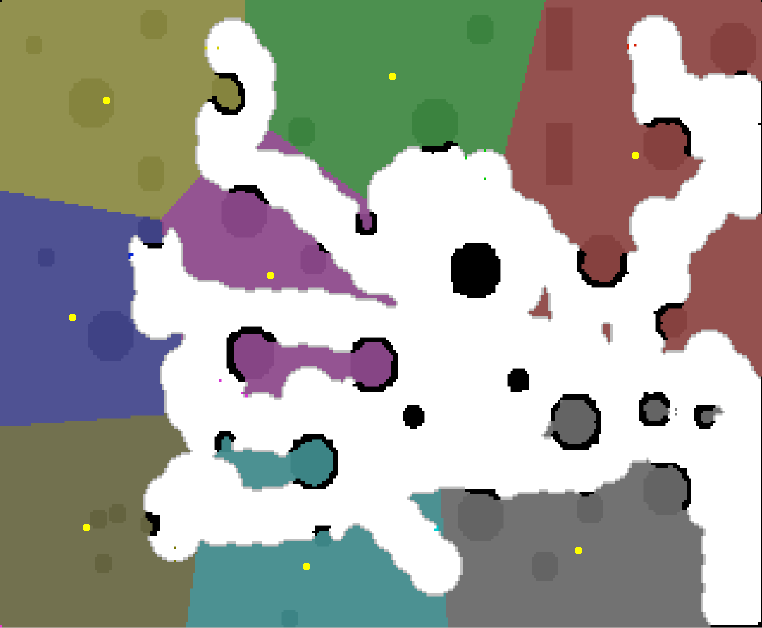
\includegraphics[width=5.5cm]{imagenes/coordGrillCM.png}
  \caption{Ejemplo de la segmentación propuesta en \cite{Solanas2004}. Extraída de \cite{wu2007voronoi}.}\label{fig:ejemploCoodGrill}
\end{figure} 

Los objetivos de exploración nuevamente serán las fronteras, la frontera $F_j$ que se asigna al robot $R_i$ es la que minimiza el $costo_{ij}$ definido en \ref{ec:costsolanas} donde $\Delta$ es una constante que representa la distancia maxima entre dos puntos del mapa (longitud de la diagonal del mapa) $||\ ||_2$ es norma euclídea, $d$ es la distancia del camino no obstaculizado mas corto entre dos celdas y $o_ij$ es una penalización acumulada que aumenta cuando $F_j$ esta en el rango de sensado de algún robot.

\begin{equation}\label{ec:costsolanas}
costo_{ij} = 
\begin{dcases}
  \Delta + || F_j - C_i ||_2 + o_{ij} & F_j \notin \zeta_i \\
  d(F_j, C_i) + o_{ij}                & F_j \in    \zeta_i
\end{dcases}
\end{equation}

Dado un robot $R_i$ la función de costo, a partir del valor $\Delta$, penaliza fuertemente a los objetivos que no pertenecen al segmento $\zeta_i$ asignado a $R_i$, por lo tanto los objetivos pertenecientes al segmento asignado al robot tendrán prioridad frente a los pertenecen a otro segmento, asegurando que los robots se mantendrán explorado sus segmentos asignados. Los objetivos pertenecientes a otros segmentos son considerados para permitir que un robot pueda continuar tomando objetivos aunque su segmento no tenga ningún objetivo restante. La penalización $o_ij$ evita el el solapamiento del los rangos de sensado de los robots, evitando así el trabajo redundante.\medbreak

Otro método es el que se describe en \cite{Lopez-Perez2018}, en este caso la segmentacion consiste en asignar cada punto del espacio desconocido a el robot mas cercano de la flota, por lo tanto el entorno se particiona en tantos segmentos $S_i$ como robots $R_i$ componen la flota de exploración. La definición exacta de los segmentos se encuentra en la ecuación \ref{ec:segmentsLopez} donde $U_i \subset M_i$ son los puntos desconocidos del espacio, $C_i$ es la posición del robot $R_i$ y la distancia $d$ se define de la misma manera que la distancia homónima del método anterior.
\begin{equation}\label{ec:segmentsLopez}
  S_i=\{c_j:d_g(C_i,c_j)\leq d(V_i(k),c_j) \forall i \neq k , c_j \in U_i\}
\end{equation}


Un ejemplo de esta segmentacion se muestra en la figura \ref{fig:ejemploCoordCenter} para un entrono completamente desconocido, donde se puede visualizar las posiciones de los robots y con colores se indican los distintos segmentos. Notar que por la definición de segmento cada robot $R_i$ se encuentra dentro del segmento $S_i$ definido a partir de su ubicación $C_i$. Otra cosa a notar sobre esta técnica de segmentacion es que en este caso, donde todo el espacio es desconocido, los segmentos se corresponden directamente a las regiones de un diagrama de Voronoi generado con las posiciones de los robots como sitios y para los casos en donde el espacio no es completamente desconocido se deberá excluir los puntos conocidos de las regiones de Voronoi para obtener la segmentacion propuesta.

\begin{figure}[H]
  \center
  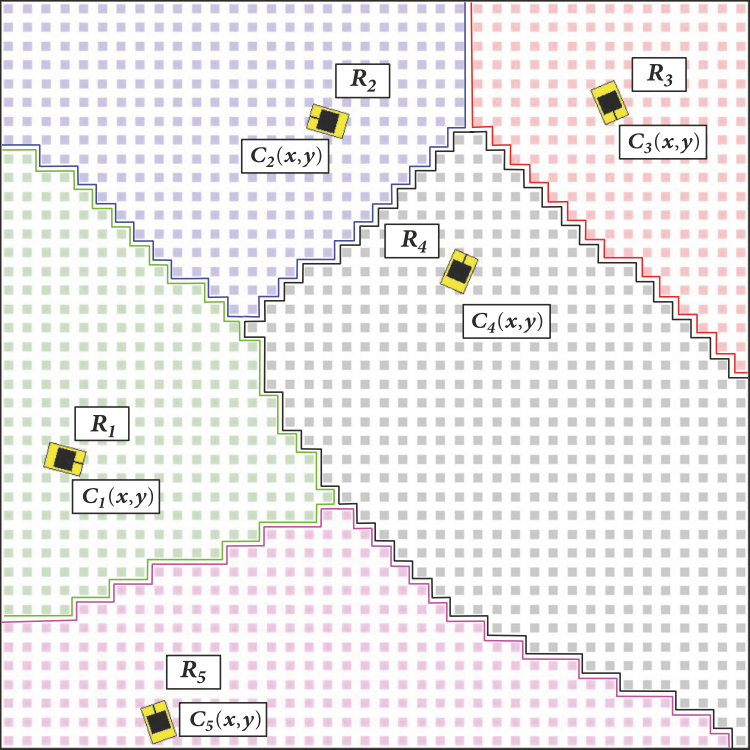
\includegraphics[width=5.5cm]{imagenes/centerCoord.png}
  \caption{Ejemplo de la segmentación propuesta en \cite{Lopez-Perez2018} y extraído de misma fuente.}\label{fig:ejemploCoordCenter}
\end{figure} 

Una vez calculados, cada segmento $S_i$ es asignado al robot $R_i$. En este método todo punto que perteneciente a algún segmento sera un posible objetivo de exploración, por lo que en este caso sera una excepción a la norma y los objetivos no serán las fronteras sino que será todo el espacio desconocido. Los robots solo pueden ser enviados a objetivos perecientes su segmento asignado, siendo el objetivo asignado el que alcanza el menor valor para la función de peso $f_p$ que se encuera definida en \ref{ec:weightLopez}.
\begin{equation}\label{ec:weightLopez}
  f_p(c_j) = k_d.d(C_i,c_j) + k_a.\phi_i(c_j)
\end{equation}
Donde $k_d$ y $k_a$ son dos constantes positivas que determinan el peso de cada sumando de la ecuación, la distancia $d$ es la definida en el método anterior, $\phi_i(c_j)$ es el angulo que queda definido entre la orientación del robot y el vector con origen en la posiciones del robot $C_i$, y fin en el centro de celda $c_j$. 

% \section{ Trabajos relacionados }
% A lo largo de esta sección se describen diferentes acercamientos para solucionar el problema de exploración multirobot. El primero es el presentado en \cite{amorin2019novel} en el cual se define un criterio para detener la exploracion multirobot basado en el concepto de ganacia de información. El siguiente, articulo \cite{wu2007voronoi} en el cual se 

\subsection{Criterio de parada}
Uno de los aspectos no mencionados hasta el momento sobre el problema de exploración es el denominado criterio de parada según el cual se determina cuando la exploración se considera finalizada. 
Una de los criterios de parada tomados usualmente es de detener la exploración cuando el mapa construido alcanza cierto un porcentaje de cubrimiento del entorno, por ejemplo 99\% \cite{Yan2015}. Esta es usualmente utilizada para evaluaciones de rendimiento donde el entorno explorado es conocido, pero no suele ser útil en práctica, ya que para utilizarse se requiere tener conocimiento previo de las dimensiones del entorno a explorar, de lo contrario es imposible saber el porcentaje de cubrimiento.

Otro posible criterio es el de explorar el entorno hasta que no quede ninguna posibilidad de obtener nueva información de el, osea que no exista ningún espacio desconocido que sea accesible. La desventaja de este criterio es que se fuerza a una exploration exhaustiva del entorno, lo cual puede ser indeseable por cuestiones de costos, tanto temporales, como de recursos como la energía de los robots, o su desgaste.

En \cite{amorin2019novel} se propone un criterio de parada que carece de la necesidad de conocer las dimensiones del entorno de antemano, haciendo factible su uso en la práctica y que a su vez evita una exploración exhaustiva. El criterio se basa en el concepto de ganancia de información que hace referencia a la cantidad de información que el robot agrega al mapa construido al completar un objetivo de exploración. 

Para experimentar y describir con detalle al criterio de parada este se define integrado a una solución en particular del problema de exploración multirobot, los aspectos de dicha solución se describen a continuación con el propósito de explicar el criterio de parada, pero también por su relevancia como ejemplo de una posible solución al problema de exploración multirobot.

El mapa es representado como una grilla de ocupación, en este contexto la ganancia de información hace referencia a las celdas del mapa cuyo contenido es determinado luego de que un objetivo es completado. 

La flota se compone de $N$ robots móviles circulares rígidos con capacidad para percibir toda la circunferencia alrededor con un radio $r$. Existe una estación central encargada de la tarea de reconocimiento de objetivos y asignación de los mismos. Los robots serán quienes recopilen la información del entorno y la central la encargada de crear un mapa global a partir de esta. Se consideran comunicaciones ideales, suponiendo que los robots no tienen restricciones de comunicación (por ejemplo, sin errores ni pérdidas con ancho de banda y alcance ilimitados). %Cabe aclarar que las comunicaciones inalámbricas son importantes en el contexto de exploración multi-robot.

Para determinar los potenciales objetivos de exploración se utiliza el concepto de fronteras, que aplicado a una grilla de ocupación se asocia a las denominadas celdas fronteras son las celdas consideradas como libres y a su vez adyacentes a celdas desconocidas. Sin embargo, se argumenta que tratar todas las celdas frontera como tareas de exploración diferentes podría ser computacionalmente prohibitivo. Por lo tanto, para reducir el costo computacional, se intenta reducir los objetivos de exploración a las celdas frontera mas representativas. Para determinar que celdas frontera serán las mas representativas, primero, las fronteras se dividen en conjuntos disjuntos $F_i$. Luego, las fronteras mas representativas de cada conjunto $F_i$ se obtienen agrupando las celdas fronteras con el algoritmo k-means con $k=\frac{|F_i|}{2r}$ donde $r$ es el radio de sensado del robots. Este proceso busca reducir los objetivos de exploración de forma de que cada frontera sea perceptible desde al menos uno de los objetivos y a su vez minimizar las celdas frontera que pueden ser percibidas desde mas de un objetivo. La figura \ref{fig:ejemploFrontSig} contiene un ejemplo de las distintas partes del proceso de extracción de fronteras significativas con $r=6.l$ siendo $l$ el largo de un lado de celda.
\begin{figure}[H]
  \centering
  \subfloat[Se identifican las celdas frotneras,  marcadas con amarillo.]{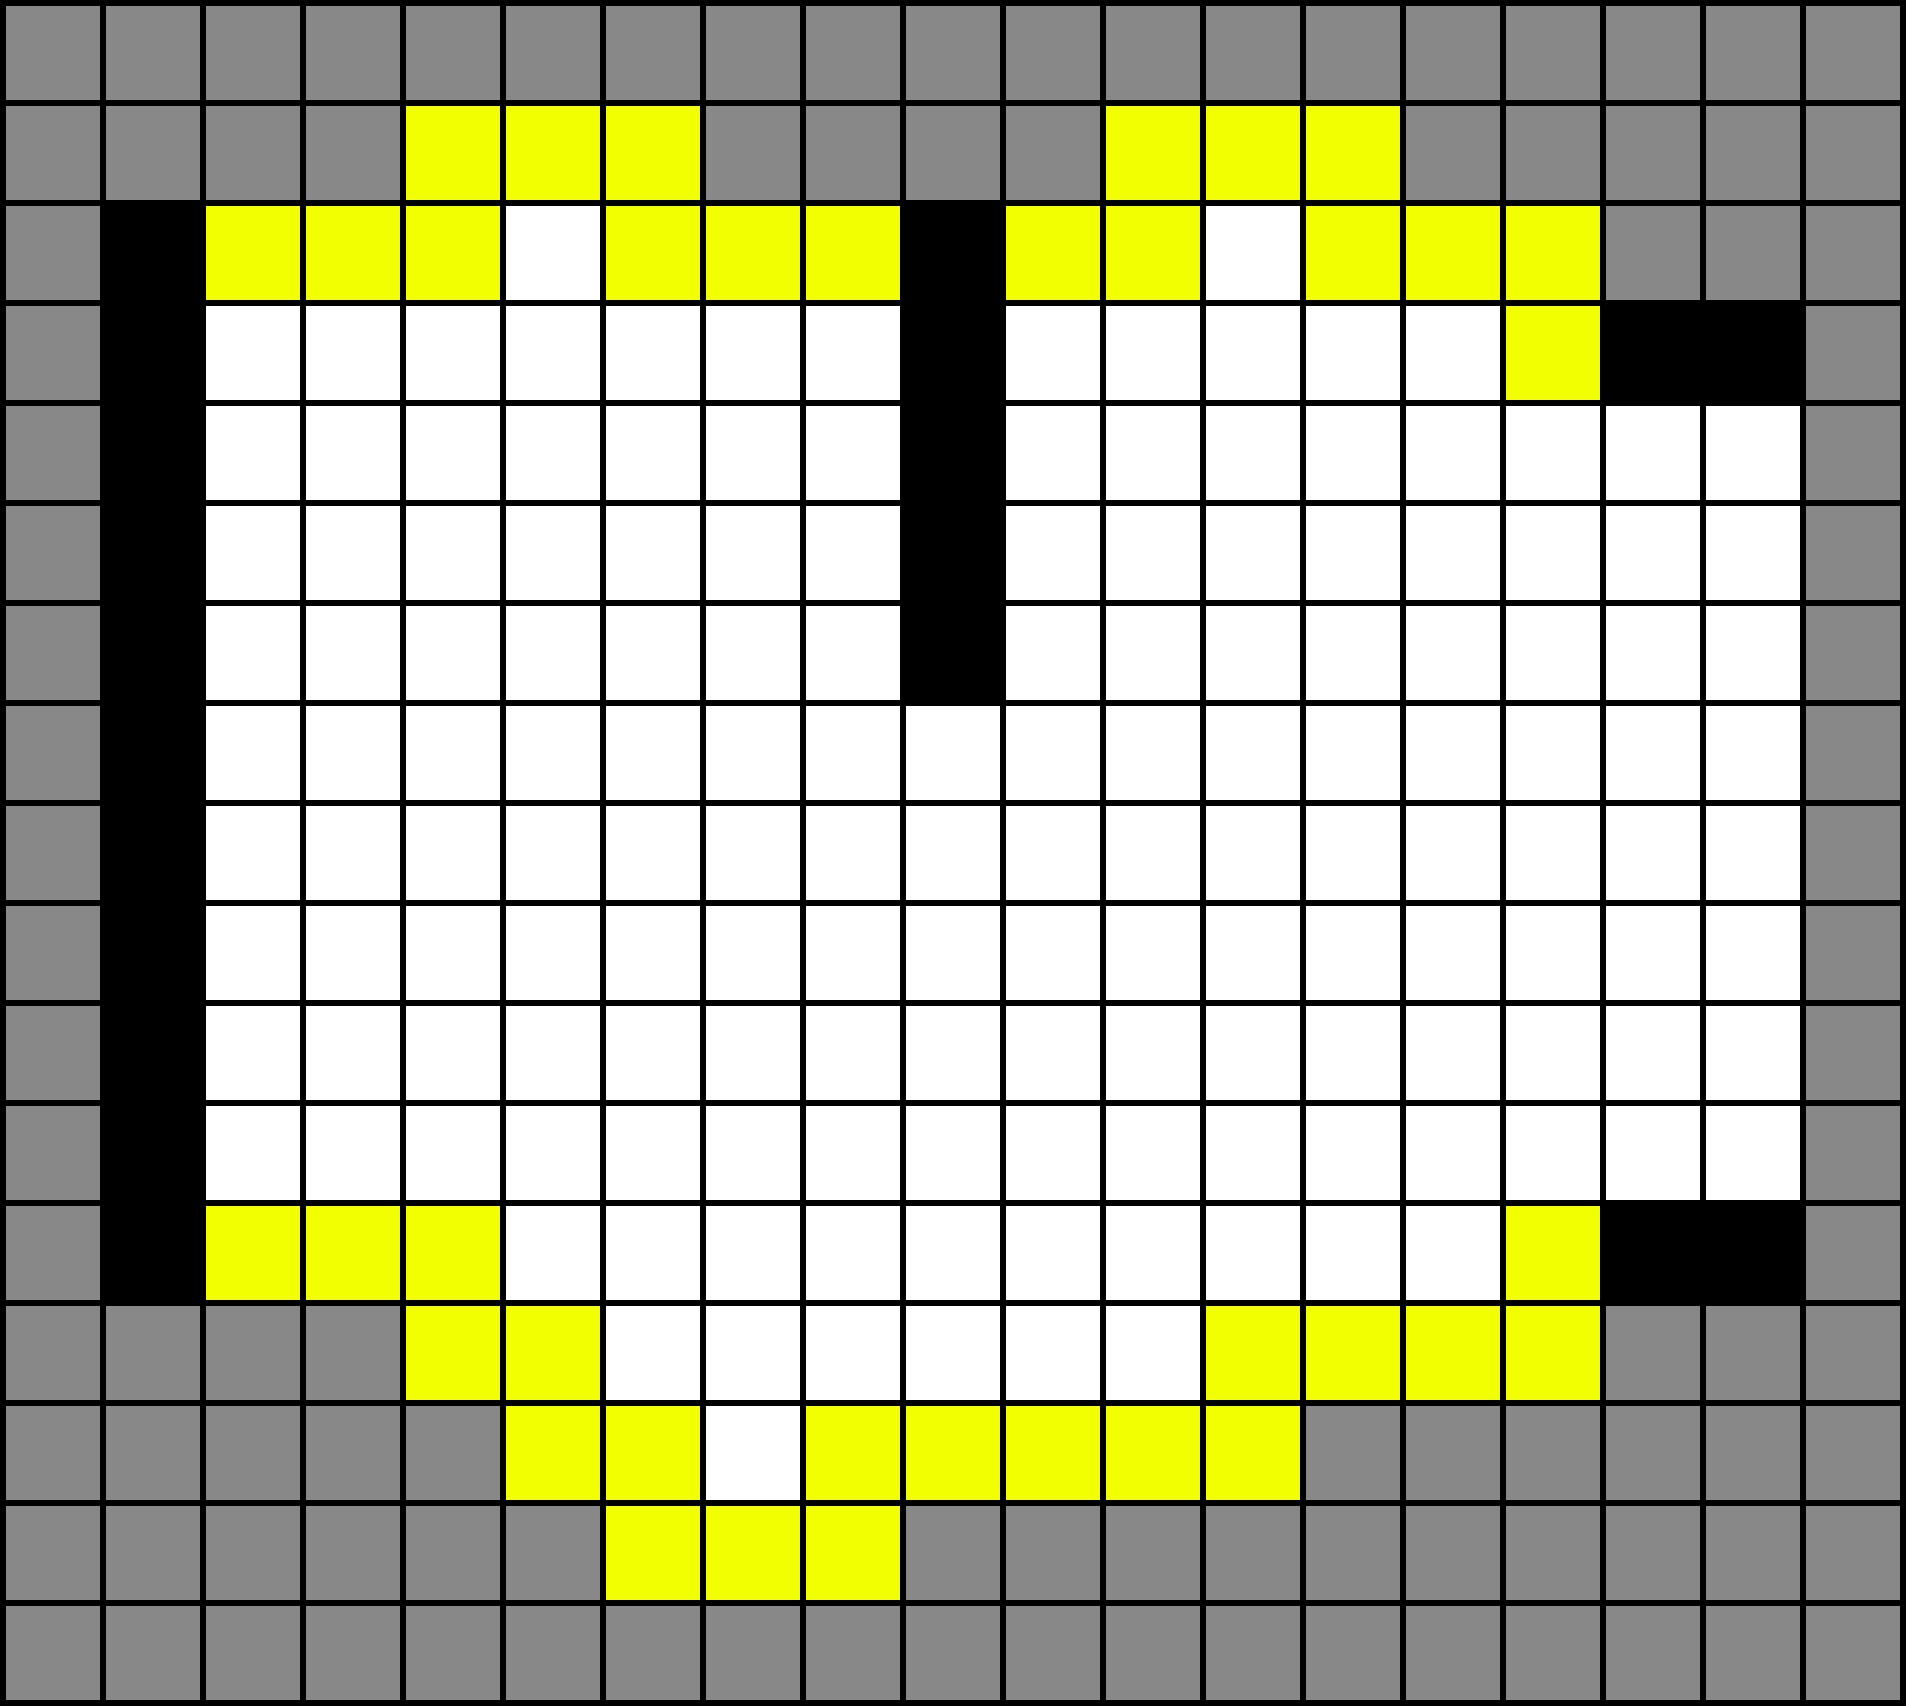
\includegraphics[clip=true, width=0.29\linewidth]{imagenes/fronterasSig/a.png}}
  \qquad
  \subfloat[Se Determinan los conjuntos de fornteras disjuntos $F_i$, cada color distinto representa un $i$ distinto.]{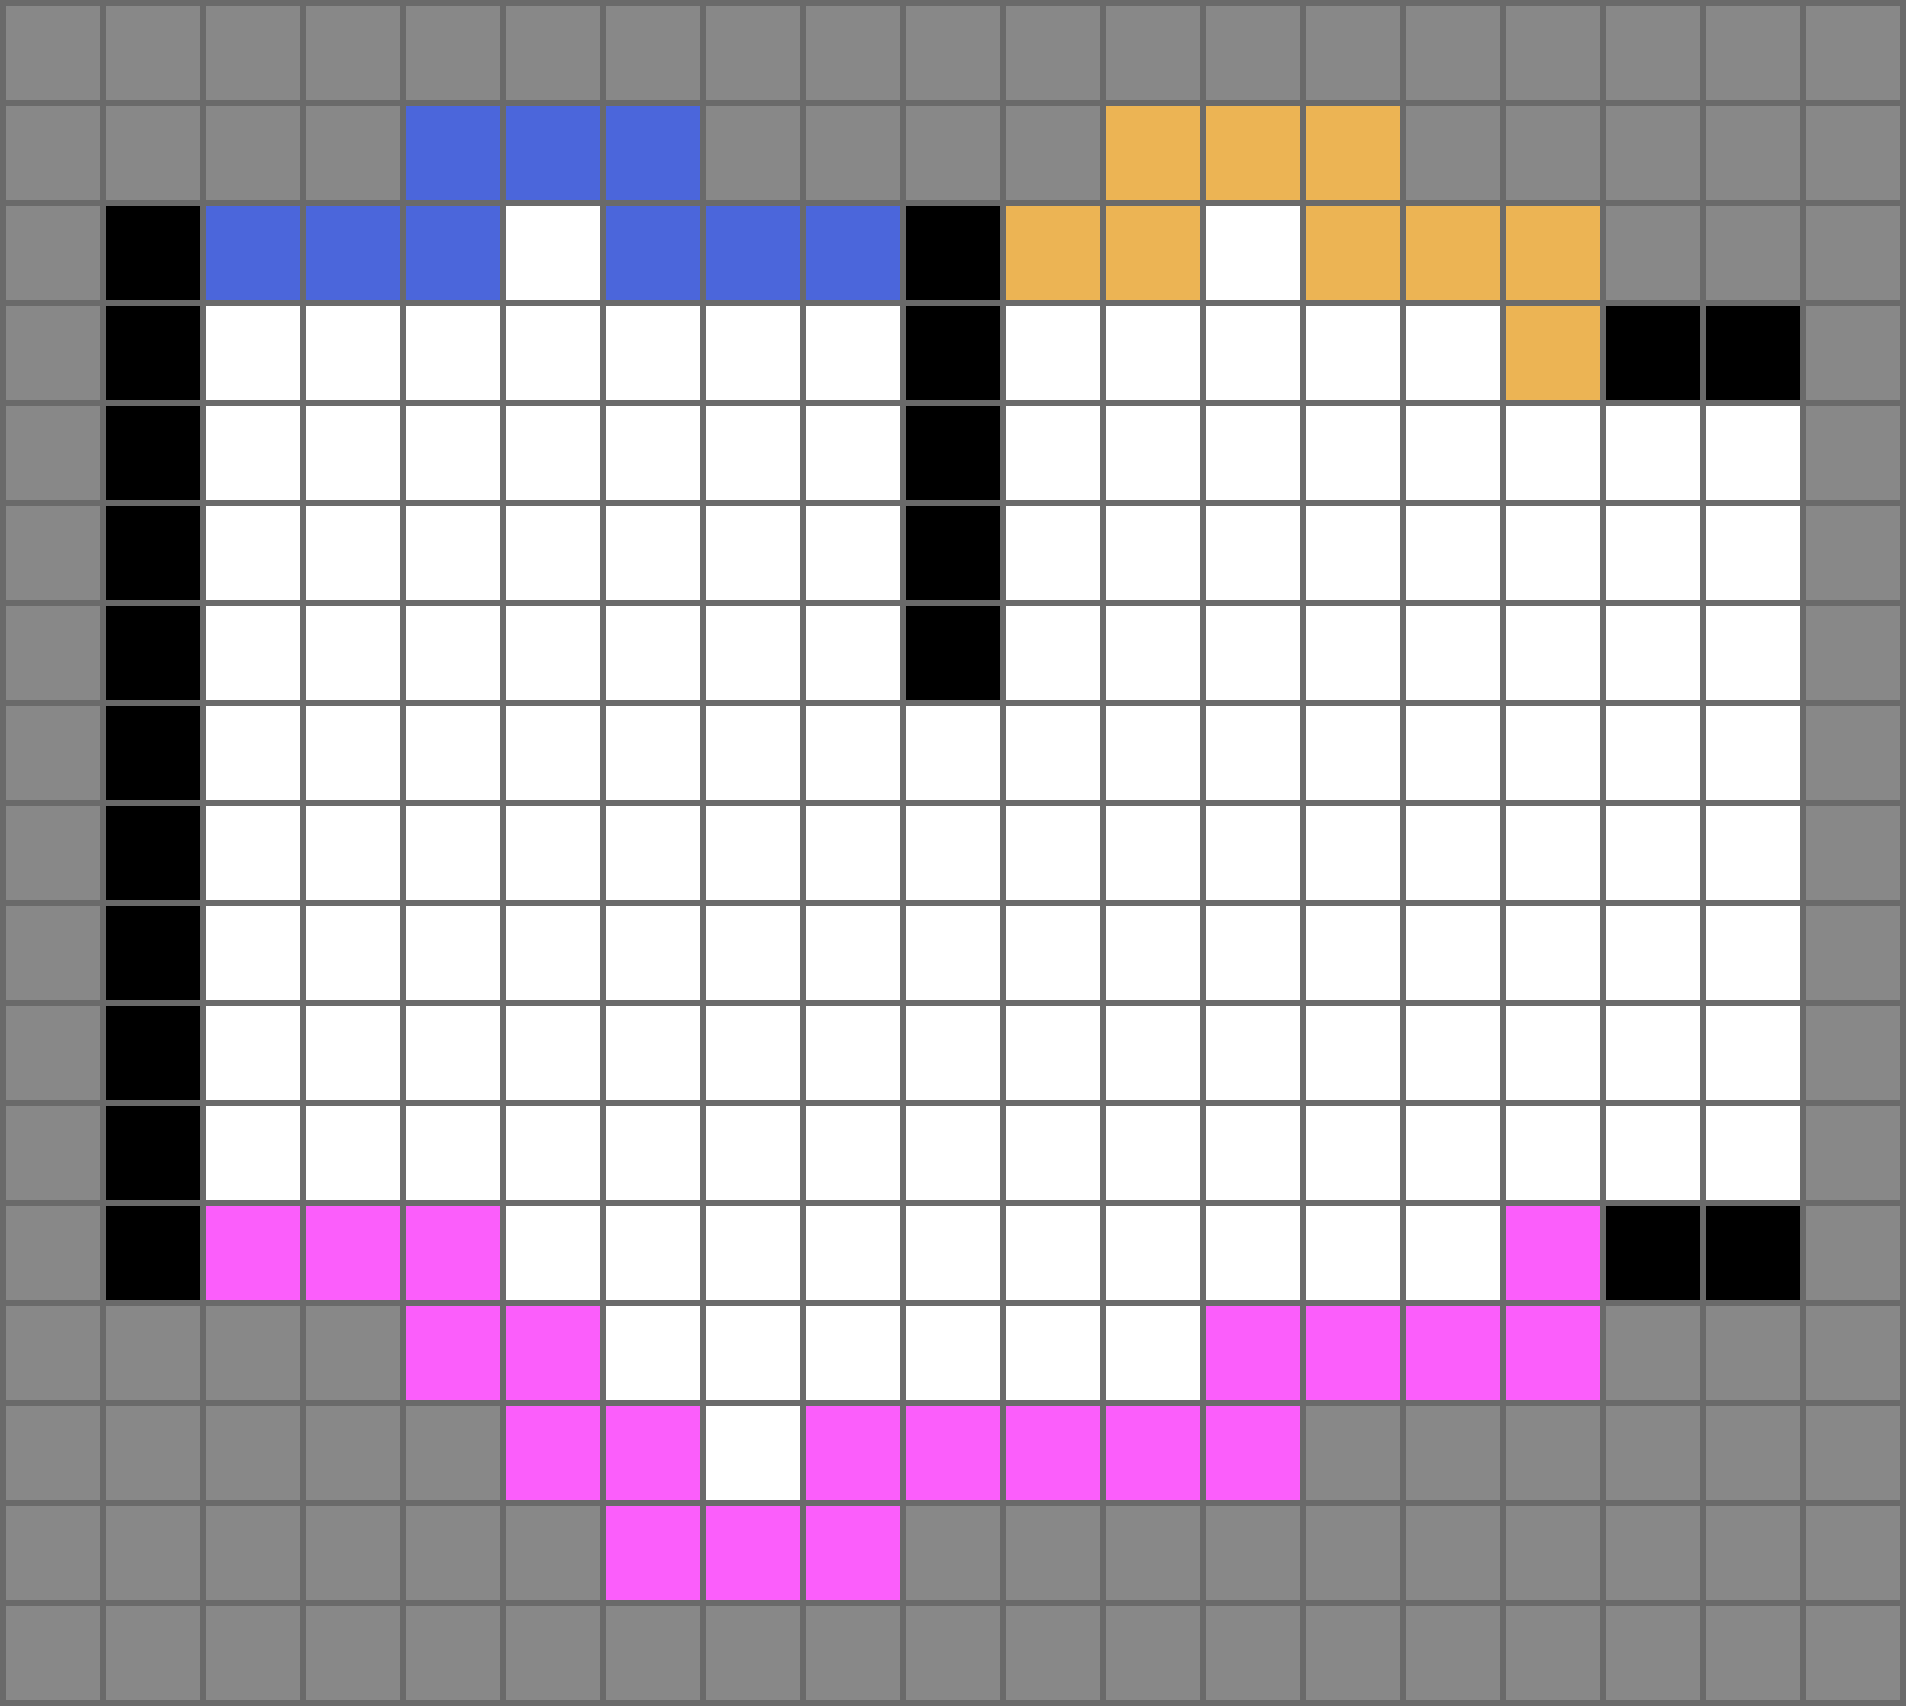
\includegraphics[clip=true, width=0.29\linewidth]{imagenes/fronterasSig/b.png}}
  \qquad
  \subfloat[Se obtienen las celdas frontera significativas de cada $F_i$ indicados con verde.]{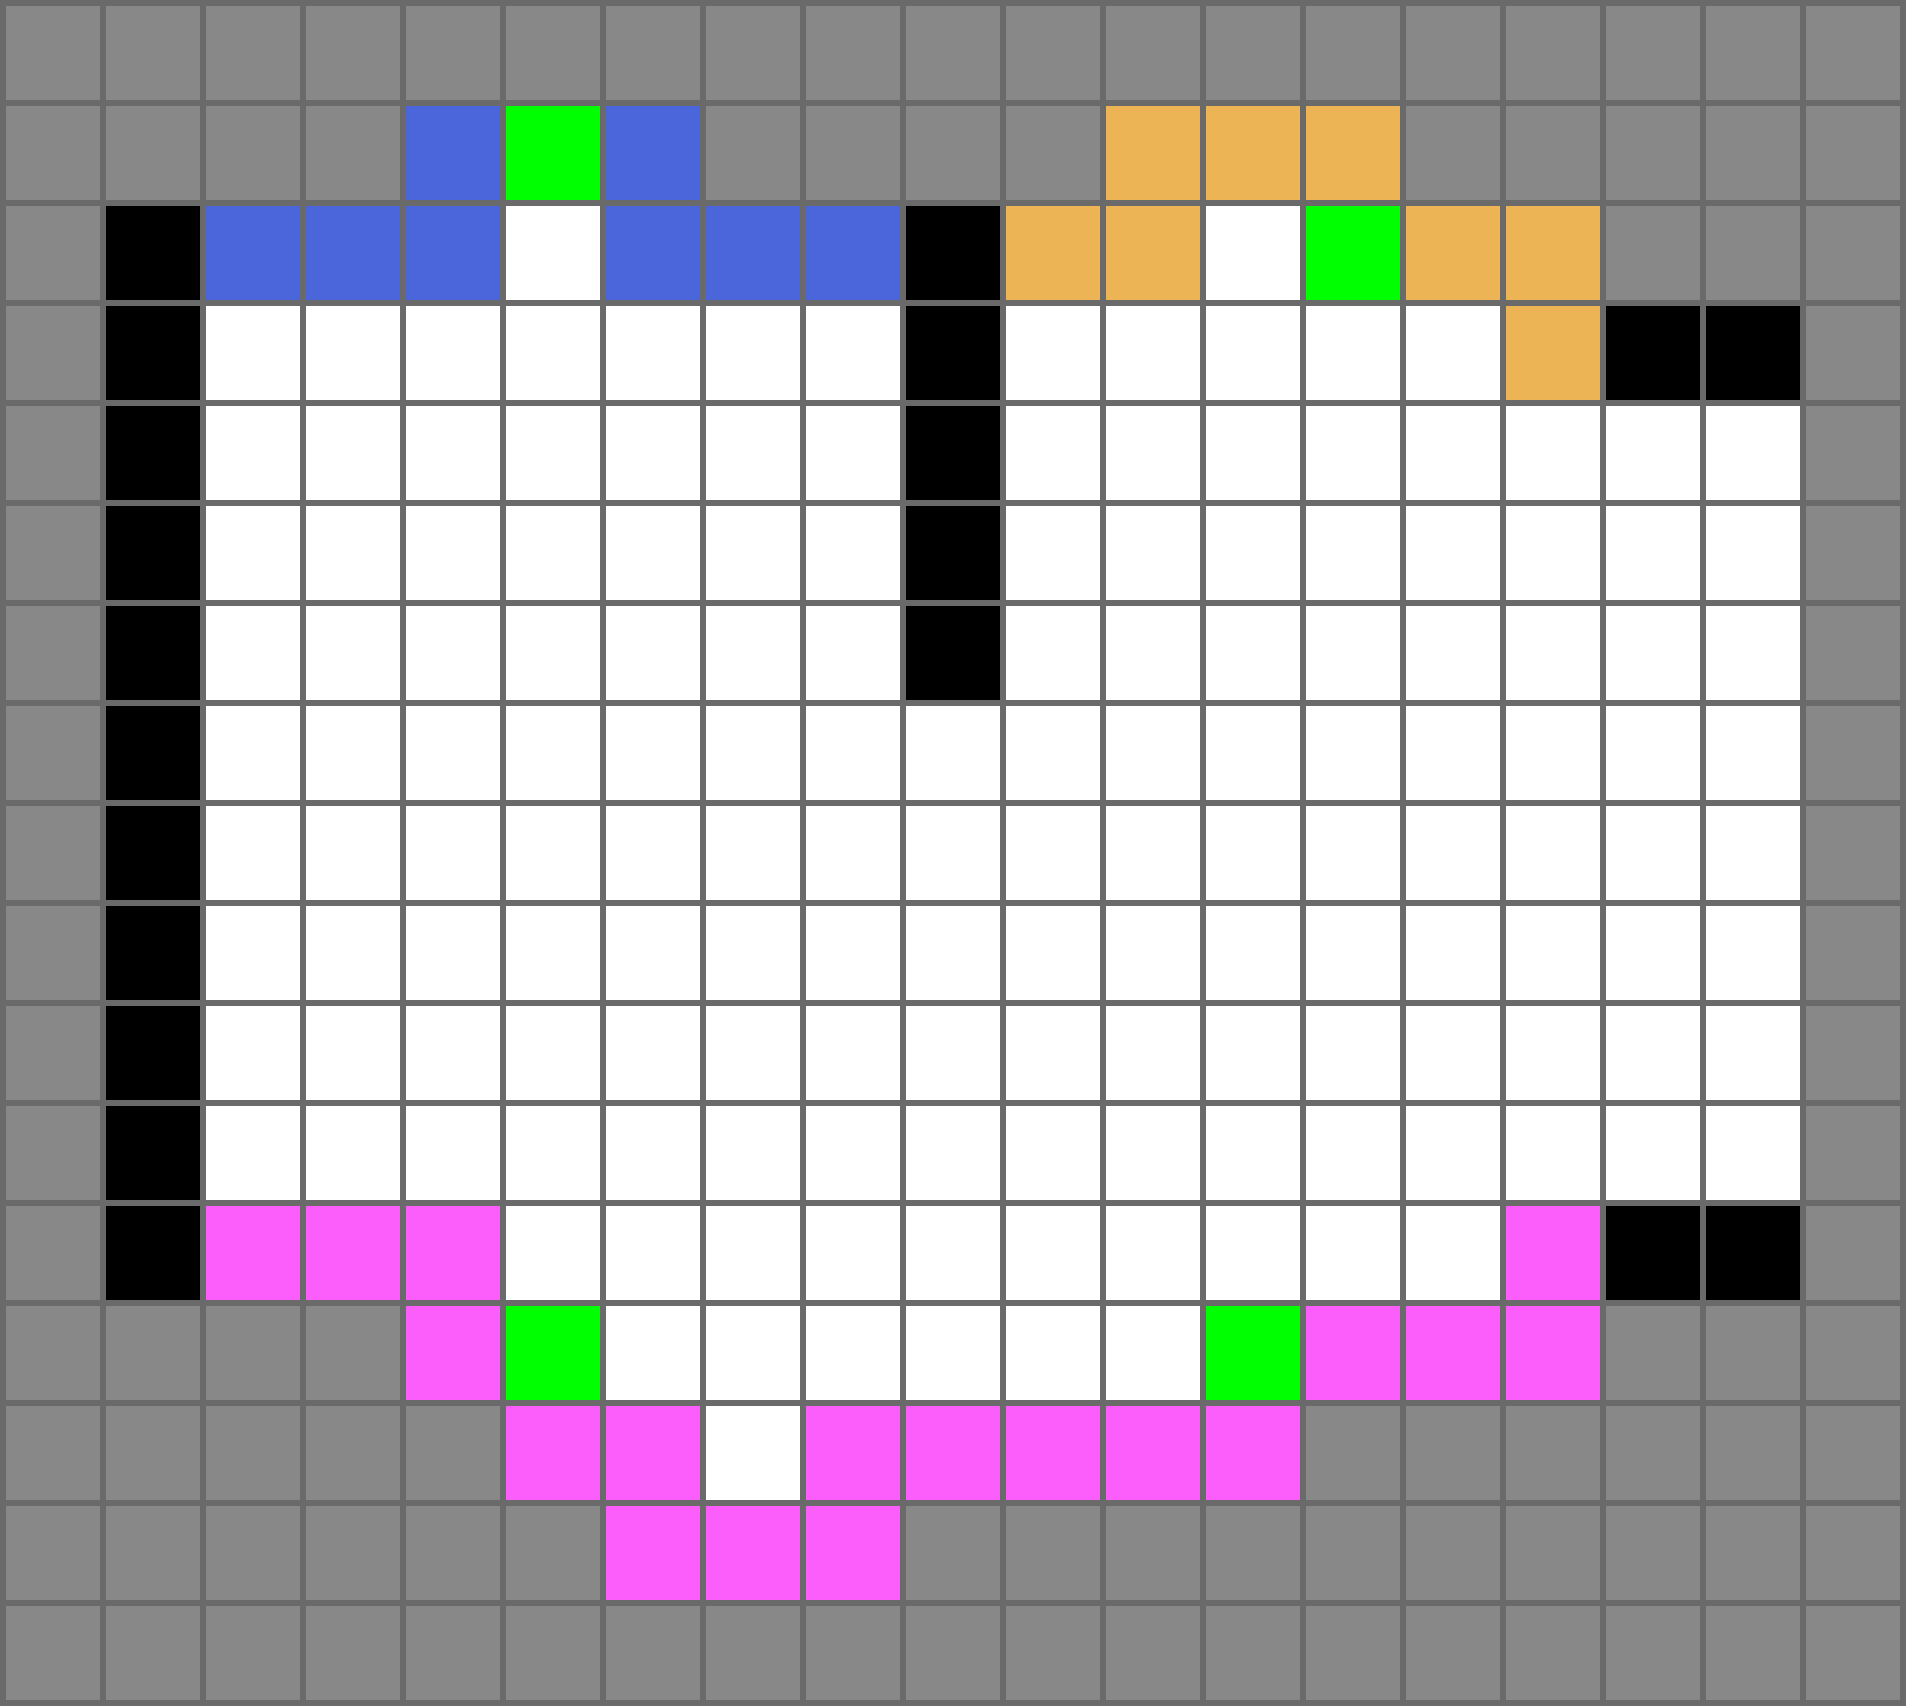
\includegraphics[clip=true, width=0.29\linewidth]{imagenes/fronterasSig/c.png}}

  \caption{Ejemplo del proceso de extracción de fronteras representativas, donde cada figura corresponde a una etapa distinta para un mismo entorno parcialmente explorado, representado con una grilla, donde las celdas blancas son libres, las negras ocupadas, y para las grises se desconoce su estado. Extraído de \cite{Amorin2019}.}\label{fig:ejemploFrontSig}
\end{figure}

La asignación de objetivos de exploración se resuelve organizando una subasta entre robots, con la estación central como mediadora, es decir, encargada de dar inicio a la subasta, recibir las ofertas de los robots, determinar los resultados de la subasta e informárselos a los robots. A continuación se detallan las etapas de una subasta.

Cuando un robot completa un objetivo de exploración (alcanza la celda frontera significativa asignada) este envía una notificación a la estación central que indica que se debe iniciar una subasta. Para dar comienzo a la subasta la estación central notifica a todos los robots sin objetivos, los cuales durante un corto período de tiempo, pueden enviar una oferta a la misma. Cada oferta consiste en una lista de pares objetivo-utilidad, donde la utilidad de un objetivo $c$ es igual a $\frac{\overline{\mli{IG}}_c}{\mli{PC}_c}$ donde $\overline{\mli{IG}}_c$ es una estimación de ganancia de información al alcanzar $c$ que se explicara más adelante y $\mli{PC}_c$ es el costo asociado a la ruta necesaria para llegar a $c$, es decir su distancia. Finalmente la central, a partir de las ofertas de todos los postores, resuelve la subasta de forma voraz, para luego notificar a cada robot su tarea asignada.

% Dada la falta de conocimiento sobre el entorno, la mejor opción para los robots es visitar los lugares donde la ganancia de información puede ser potencialmente mayor, sin dejar de considerar el esfuerzo necesario llegar al objetivo, por lo tanto, los robots priorizarán las tareas por el coeficiente entre la ganancia de información esperada y el esfuerzo esperado necesario para completar la tarea.

La ganancia de información estimada que es utilizada en el calculo de la utilidad y en el criterio de parada que se presentara a continuación, se calcula según la ecuación \ref{ec:infGain}. 
%varios conceptos.  Para cada celda $c$ de la grilla de ocupacion las coordenadas $(x_c,y_c)$ son las correspondientes al centro de la celda $c$.
\begin{equation}\label{ec:infGain}
  \overline{\mli{IG}}_c = \overline{\mli{IG}}_{(x_c,y_c)} = |{c_i}|
\end{equation}
Donde toda celda $c_i$ cumple con:
\begin{enumerate}[label=(\roman*)]
  \item $c_i$ es una celda desconocida.
  \item $c_i$ se puede percibir desde $c$:
  \begin{itemize}
    \item $c_i$ esta en rango del sensor desde $c$: $\sqrt{(x_c - x_{c_i})^2 + (y_c - y_{c_i})^2}\leq r$
    \item No existe celda $c_o$ obstaculizada que obstruya a $c_i$ desde $c$:\\
      $\nexists\ c_o \ obstaculizada \ \land \ \frac{ |(\frac{y_{c_o}-y_c}{x_{c_o}-x_c})(x_{c_i}-x_c) - y_{c_i} - y_{c}| }{\sqrt{(\frac{y_{c_o}-y_c}{x_{c_o}-x_c})+1}}\leq \delta $
  \end{itemize}
\end{enumerate}

Siendo el valor $\delta$ igual a la mitad de longitud diagonal de una celda, por ser este la maxima distancia que puede existir entre una celda obstaculizada $c_o$ y el segmento de recta definido entre $c$ y $c_i$ sin que $c_o$ obstruya a $c_i$ desde $c$. En la figura \ref{fig:ejemploOclusionAm} se muestra un ejemplo de celdas que cumplen con las condiciones antes mencionadas y celdas que las cumplen, haciendo énfasis en dos celdas particulares una obstruida y otra no obstruida.

\begin{figure}[H]
  \centering
  \subfloat[La celda con sus centro indicado en azul se puede precibir, esta dentro del rango del sensor y no existe un obstaculo que la obstruya.]{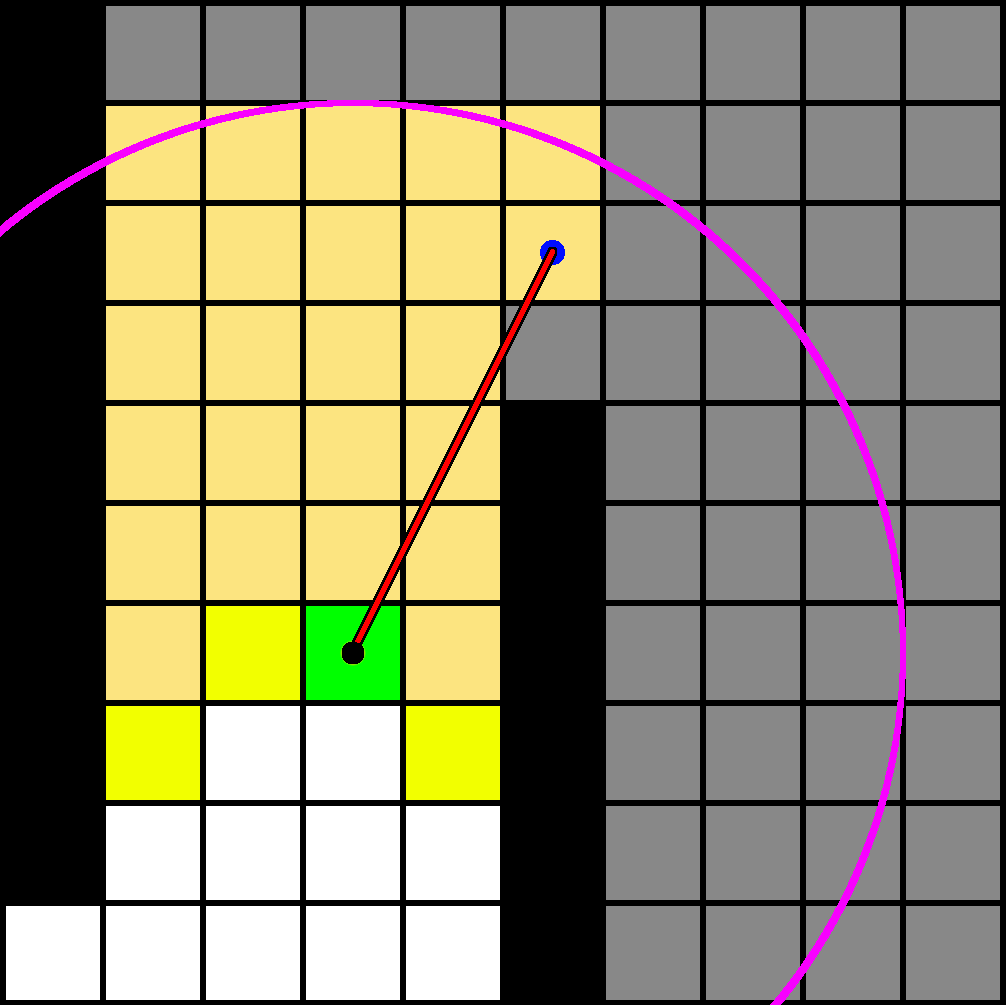
\includegraphics[clip=true, width=0.47\linewidth]{imagenes/oclusion/a.png}}
  \qquad
  \subfloat[La celda con su centro indicado en azul \textbf{no} se puede precibir, esta dentro del rango del sensor pero existe un obstaculo que la obstruye.]{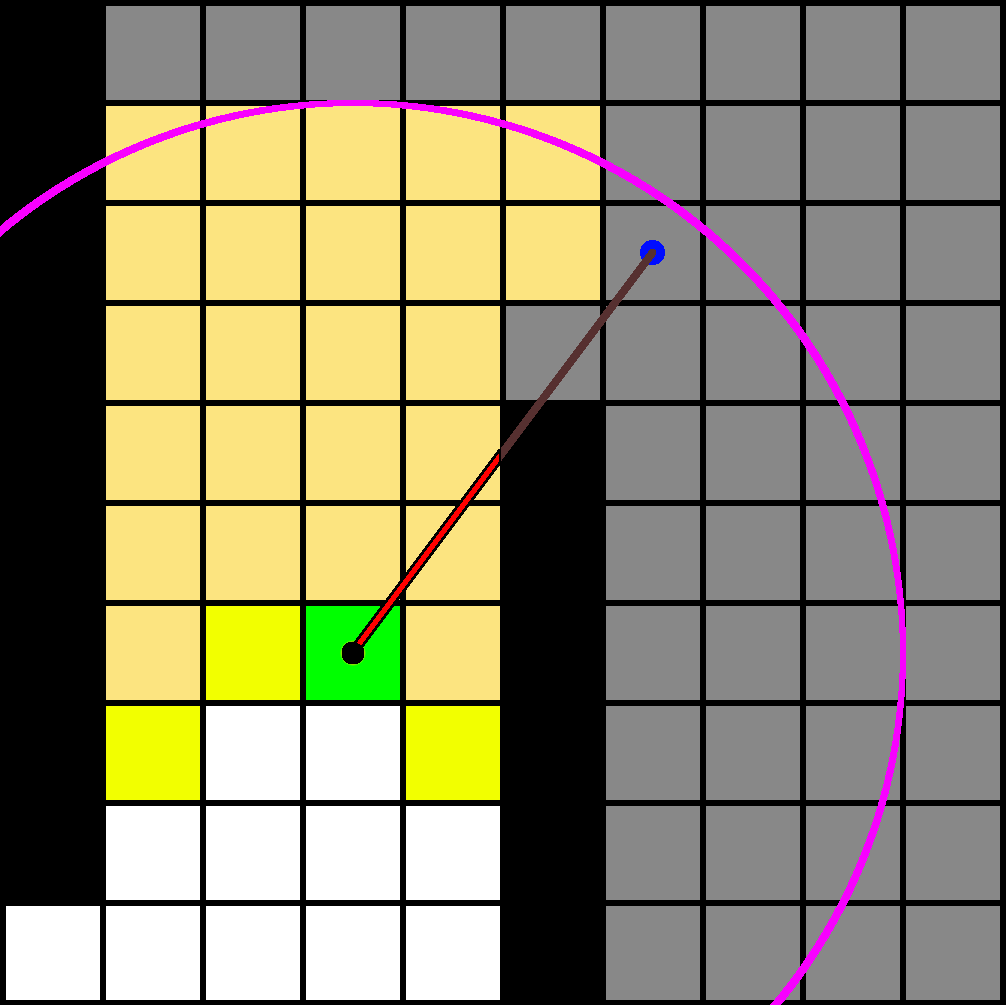
\includegraphics[clip=true, width=0.47\linewidth]{imagenes/oclusion/b.png}}

  \caption{Ejemplo de las condiciones que debe cumplir una celda para contabilizar en el calculo de la ganancia de información. Lo representado por las celdas blancas, grises, negras, verdes y amarillas coincide con lo que estas representan en la figura \ref{fig:ejemploFrontSig}. Las condiciones se comprueban tomando la celda cuyo centro se marca con un punto negro como la celda $c$ y las celdas que cumplen con las condiciones se colorean con naranja. Extraído de \cite{Amorin2019}.}\label{fig:ejemploOclusionAm}
\end{figure}



 % esto mejora sus habilidades para predecirlo de forma continua hasta que sus habilidades de predicción serán lo suficientemente buenas
El criterio de parada propuesto en el articulo, se basa en la idea de que durante la exploración los robots obtienen conocimiento sobre el entorno, y que llegado un punto su conocimiento sobre el entorno sera lo suficientemente bueno como para estimar el estado de las zonas desconocidas del mapa de forma precisa.

Teniendo en cuenta que una suposición básica es que la flota explora entornos limitados, las hipótesis necesarias para que el criterio de parada propuesto sea valido son dos. La primera es que existe un momento a partir del cual la estimación de la ganancia de información se puede hacer con precisión (es decir, el error cometido por el estimador tiende a cero). Y la segunda es que dicho momento puede determinarse en línea mediante robots que calculan su propio error en sus estimaciones de ganancia de información. 

El criterio de parada consiste en finalizar la exploración cuando todos los robots, de forma independiente, determinan concluir su participación en la exploración. El criterio que un robot individual usa para determinar cuando debe dejar de explorar, es el de tener $\eta$ predicciones acertadas. Dado un umbral de tolerancia $\chi$ una una predicción es acertada cuando, al completar objetivo $c$ la diferencia entre la estimación de ganancia de información $\overline{\mli{IG}}_c$ y la ganancia de información real $\mli{IG}_c$ es menor a $\chi$ (ecuación \ref{ec:sthit}). 
\begin{equation}\label{ec:sthit}
  |\overline{\mli{IG}}_c - \mli{IG}_c| \leq \chi
\end{equation}
La idea subyacente de este criterio es al experimentar $\eta$ predicciones acertadas un robot tiene la suficiente información sobre el entorno como para poder estimar la porción inexplorada con precisión, y por lo tanto podrá detenerse.

% \subsection[Voronoi-Based Space Partitioning for Coordinated Multi-Robot Exploration]{Voronoi-Based Space Partitioning for Coordinated\\ Multi-Robot Exploration} 
\subsection{Mapa métrico basado en polígonos}
% Este artículo describe y evalúa la extensión de un algoritmo de exploración multi-robot y muestra que al reemplazar el modelo de mapa original (una grilla de ocupación) con una representación poligonal más compacta y flexible, el nuevo enfoque aumenta significativamente la eficiencia de la etapa más costosa del algoritmo original, que es la división de áreas desconocidas en tantas regiones como robots. El algoritmo de agrupación K-Means original se sustituye por un algoritmo de partición basado en Voronoi aplicado a polígonos.
Las grillas de ocupación son de los mapas métricos mas utilizadas en el contexto de exploración multirobot, sin embargo, estas grillas no son apropiadas para entornos que son muy grandes o cuyos límites no están bien delimitados desde el comienzo de la exploración. En contraste, las representaciones poligonales no tienen tales limitaciones.

El artículo \cite{wu2007voronoi} propone utilizar una representación poligonal en la cual el mapa consiste en la union de conjunto de polígonos cerrados de forma y tamaño arbitrario, que pueden estar libres, no explorados u obstaculizados. 

Para comprobar y validar la representación propuesta se adapta la estrategia de exploración multirobot presentada en \cite{Solanas2004} (cuya técnica de coordinación fue mencionada en \ref{subsec:coordNoTop}) que originalmente se basa en grillas de ocupación, para que funcione utilizando una representación poligonal.

De las pruebas realizadas los autores concluyen que una representación poligonal es más compacta, flexible y logra aumentar significativamente la eficiencia.

% El desempeño de la representación propuesta se comprueba a partir de implementar una estrategia de exploración multirobot que adapta  una estrategia de exploración multirobot que hace uso de grillas de ocupación\cite{Solanas2004}, de lo cual se concluye que una representación poligonal es más compacta, flexible y logra aumentar significativamente la eficiencia.

\subsubsection{Representación poligonal}
Inicialmente, todo el mapa estará constituido por un solo polígono desconocido. A partir de lo sensado por cada robot, se incluye nueva información sobre entorno a la representación agregando polígonos libres y ocupados que son substraídos de los polígonos desconocidos a los que pertenecían.

Los objetivos de exploración se determinan a partir de las aristas entre polígonos desconocidos y polígonos libres denominadas como aristas frontera que son análogas a las celdas frontera de las grillas de ocupación.

El trabajo propone asignar tareas a partir de la division el entorno desconocido en tantas regiones como robots existan en la flota, para luego asignar a cada robot la tarea de explorar una region diferente. El entorno se divide a partir de un algoritmo que adapta al algoritmo K-Means para funcionar a partir de la representación poligonal propuesta, este algoritmo se explica en la sección\ref{subsubsec:particionamientovoronoi}.

%La division del entorno se logra adaptando el algoritmo K-means para funcionar en utilizado para encontrar los centroides correspondientes a las agrupaciones de áreas desconocidas, ya que se asume que estos serán los puntos más provechosos para que los robots exploren.

Finalmente, la planificación del camino del robot es realizada en el interior de los polígonos libres, cosa que se puede hacer a partir de la aplicación de cualquier algoritmo de descomposición celular, por ejemplo el que se explica en \cite{schachter1978decomposition}.
   
\subsubsection{Particionamiento basado en polígonos}\label{subsubsec:particionamientovoronoi}
El diagrama de Voronoi\cite{fortune1987sweepline} de un conjunto de puntos 2D, también conocidos como sitios, $C_{i} , 1 \leq i \leq K$, es una partición de ese espacio en $K$ regiones convexas disjuntas conocidas como células Voronoi. Cada región $V_i$ está definida por los puntos en el espacio que están más cerca de $C_{i}$ que a cualquier otro $C_{j}$, $j\neq i$. 

Sea $n$ numero de robots, el resultado deseado es obtener un conjunto de $K=n$ celdas de Voronoi para las cuales, sus centroides (centros de masa) y sus sitios estén a una distancia menos que cierta tolerancia $\varepsilon$. % cerradas que están globalmente delimitadas por el polígono a dividir

La generación de estas celdas se realiza a partir del algoritmo \ref{alg:particionamientovoronoi} que adapta, utilizado diagramas de Voronoi, al algoritmo K-Means utilizado en la implantación base, que no es compatible con una representación poligonal.

\begin{algorithm}
\SetAlgoLined
    Elegir aleatoriamente $K$ puntos $C_i$, $1 \leq i \leq K$, contenidos en los polígonos correspondientes a las regiones desconocidas actuales en el mapa.\\
    Calcular el diagrama de Voronoi asociado con el conjunto actual de $C_i$.\\
    Restringir las celdas del diagrama de Voronoi a los polígonos desconocidos actuales.\\
    Determinar el centro de masa $M_i$ de cada celda Voronoi restringida.\\
    \eIf{$C_i - M_i < \varepsilon\ \forall i$}{
        Saltar al paso 11.\\
    }{
        Sustituir cada $C_i$ por su $M_i$ correspondiente.\\ Volver al paso 2.\\
    }
    
    Dividir el conjunto de polígonos desconocidos en $K$ regiones disjuntas según las celdas de Voronoi restringidas encontradas.\\
    \caption{Particionamiento basado en Voronoi}
    \label{alg:particionamientovoronoi}
    
\end{algorithm}

Notar que el algoritmo trabaja con celdas de Voronoi restringidas, estas son las celdas resultantes de un diagrama de Voronoi restringidas a los limites del mapa conocidos por hipótesis.


%%%%%%%
% Desde acá proyecto de grado redactado
%%%%%%%

% \subsection[Distributed Multi-robot Exploration Based on Scene Partitioning and Frontier Selection]{Distributed Multi-robot Exploration Based on\\ Scene Partitioning and Frontier Selection}
\subsection{Exploración multirobot distribuida} 
% Al considerase una solución para el problema de exploración hay dos aspectos centrales a resolver, identificar posibles objetivos de exploración y como priorizar estos objetivos de forma de priorizar los mas relevantes.

En \cite{Lopez-Perez2018} se propone una solución completamente distribuida al problema de exploración multirobot. Este tipo de resolución implica descentralización, lo que aumenta tanto la robustez del sistema como su autonomía en tanto solo se requiere del equipo robótico para explorar el entorno, sin depender de una entidad central para coordinar ningún aspecto de la solución. %, que al igual que otras ya comentadas partición el entorno aunque en este caso dicha 

\subsubsection{Formulación del problema}
La variante del problema de exploración multi-robot tratada en este articulo es la de explorar un entorno desconocido $W\in R^2$ utilizando un conjunto de robots $R={R_1,R_2,...,R_n}$. Se utiliza una grill  de ocupación, por lo que el entorno se descompone en un conjunto de celdas $C={c_1,c_2,...,c_n}$. Cada robot $R_i$ posee: 
\begin{enumerate}
  \item Un mapa $M_i \in CxL$ donde $L$ son las diferentes estados en los que puede estar una celda. 
  \item Una posición inicial $q_{init}^{i}\in R^2 \times [-\pi,\pi]$. 
  \item Un sensor $S_i$ para explorar el entorno desconocido.
\end{enumerate}

Adicionalmente se asume que existe siempre un cuadro delimitador de $W$ que puede ser establecido, aunque sea de forma aproximada, antes de que la exploración comience, comunicación perfecta (sin perdida y de rango infinito) y que cada robot tiene acceso a su posición respecto a un marco de referencia común.

\subsubsection{Descripción del sistema}
El sistema tiene un diseño modular, este consta de 4 módulos que se encuentran replicados en cada robot, el modulo de distribución de información, el modulo de asignación de zonas, el modulo de adquisición de información y el modulo de exploración. Estos se describen en las siguientes secciones. 

\paragraph{Modulo de distribución de información}
Este modulo se encarga de distribuir a los demás robots la posición del robot al que pretence, las ubicaciones que conoce de los demás robots y su mapa $M_i$. 

\paragraph{Modulo de asignación de zonas }
El entorno es segmentado en zonas y la exploración cada una de estas es asignada a un robot. El modulo de asignación de zonas es el responsable de realizar la segmentación en zonas y su posterior asignación a los robots. La segmentación genera tantas zonas $E_i$ como robots $R_i$ que $E_i$ se define en la ecuación \ref{ec:zones} a partir de la posición $C_i$ de $R_i$. .
\begin{equation}\label{ec:zones}
  E_i=\{c_j:d_g(C_i,c_j)\leq d_g(V_i(k),c_j) \forall i \neq k , c_j \in U_i\}
\end{equation}
Donde $U_i \subset M_i$ son la celdas desconocidas del mapa asociado al robot $R_i$ y $d_g(c',c'')$ es la distancia geodésica, que indica el camino compuesto de centros de celdas mas corto entre dos celdas $c'$ y $c''$ que respecta la conectividad entre las celdas que lo componen.

Cada zona $E_i$ es asignada al robot $R_i$ y este explorara las celdas de $E_i$ según lo determine el \hyperref[par:estar:moduloexp]{modulo de exploración}.

\paragraph{Modulo de adquisición de información}
El propósito de este es el de actualizar el mapa $M_i$ de el robot $R_i$ según la información obtenida por su sensor $S_i$ y su posición $C_i$.

\paragraph{Modulo de exploración}\label{par:estar:moduloexp}
El modulo de exploración esta compuesto por tres submódulos. 

El primero de ellos es el submódulo de asignación de objetivos, como su nombre lo indica, este se encarga de seleccionar un objetivo de todos los pertenecientes a la zona asignada $E_i$ para asignarlo al robot $R_i$. El objetivo seleccionado $G_i$ es el que alcanza el menor valor para la función de peso $f_p$ que se computa como \ref{ec:weight}.
\begin{equation}\label{ec:weight}
  f_p(c_j) = k_d.d_g(C_i,c_j) + k_a.\phi_i(c_j)
\end{equation}
Donde $k_d$ y $k_a$ son dos constantes positivas que determinan el peso de cada sumando, $d_g(C_i,c_j)$ hace referencia a la distancia geodésica mencionada anteriormente, $\phi_i(c_j)$ es el angulo entre la orientación del robot y el vector con origen en la posiciones del robot $C_i$, y fin en el centro de celda $c_j$. 

Luego esta el submódulo de planificación de ruta, este se encarga de generar una ruta que le permita al robot llegar al objetivo asignado. Esto se logra a partir del algoritmo $A*$, para la ejecución de este se asume que las celdas desconocidas son libres. En el caso de encontrarse un obstáculo en la ruta planificada se replanifica ejecutando nuevamente el algoritmo $A*$ en la version mas reciente del mapa.

El ultimo es el submódulo de ejecución de trayectoria que se encarga de generar los comandos de actuación para seguir una ruta planeada.

% \subsection[semi-structured]{Incremental Topological Segmentation for Semi-\\structured Environments using discretized GVG}

% Este articulo se centra en la descripción de un método de segmentación incremental del entorno que se basa en la propuesta por Thrun \cite{Thrun1998}. Para lograr la incrementalidad se desarrollaron variantes incrementales para la generación del GVD y para la detección de segmentos.

% El algoritmo de generación incremental del GVD se basa en el desarrollado en \cite{kalra2009incremental}. 

% La detección incremental de puntos críticos se hace solo considerando la definición básica de Thrun, sin considerar las técnicas de remoción de falsos positivos propuestas por Wurm \cite{wurm2008coordinated}, esto facilita la tarea de detección pero impacta negativamente los resultados. Para lograr la mencionada detección incremental de puntos críticos, se recalculan los mínimos locales según los cambios del GVD (nuevos nodos, nodos removidos, cambios de despeje) de cada incremento, específicamente se recalcula en los cambios y sus vecinos de primer y segundo grado. Al detectar nuevo punto critico se calcula la linea critica asociada.

% Finalmente es necesario, a partir de las lineas criticas, determinar de forma incremental a que segmento pertenece cada celda. Para esto, se elije una celda de todas las celdas afectadas en el incremento y se la agrega a una nueva region, sus celdas vecinas que estén dentro del mapa, no estén ocupadas y no sean cruzadas por una linea critica serán agregada...

% % \begin{algorithm}
% % \SetAlgoLined
% %     Determinar segmentos $S = \{s_{1} , ..., s_{n} \}$ del mapa\\
% %     Determinar el conjunto de fronteras objetivo para cada segmento\\
% %     \For{cada robot $i$}{
% %         \For{cada segmento $s \in S$}{
% %                 Computar el costo $C_{s}^{i}$\\
% %                 Descontar al costo $C_{s}^{i}$ si el robot $i$ ya se encontraba en $s$\\
% %             }
% %     }
% %     Asignar robots a los segmentos usando el método húngaro\\
% %     \For{cada segmento $s \in S$}{
% %         Asignar robots a las fronteras objetivas en $s$ utilizando el método húngaro\\
% %     }
% %     \caption{Asignación de objetivos}
% %     \label{alg:asignacionobjetivos}
    
% % \end{algorithm}


% hasta acá redactado


% \subsection[Incremental contour-based topological segmentation for robot exploration]{Incremental contour-based topological\\ segmentation for robot exploration}
% \subsubsection{Resumen}
% Habla de mapas topológicos, estos son los mapas que se generan a partir de la segmentación del entorno. 
% Específicamente se centra en describir y evaluar un algoritmo de segmentación para la contracción de mapas topológicos en 2D: Segmentación topológica basada en el contorno de los obstáculos del mapa (Contour Based Topological Segmentation).
% También se describe una variante incremental para poder usarse en tiempo real para la exploración multi-robot.

% \subsubsection{Notas generales}
% Interesante tener en cuenta la existencia de diferentes métodos para segmentar el espacio.

% Este se evalúa contra la segmentación humana.

% Se describe una variante incremental para poder usarse en tiempo real para la exploración multi-robot.

% En la parte de trabajos relacionados habla de la segmentación basada en GVD. <- importante

% Interesante el trabajo relacionado por describir los tipos de segmentación

% Funcionamiento:
% \begin{enumerate}
%   \item De grid 2D based map a un conjunto de polígonos:
%   \begin{enumerate}
%      \item De grid a imagen binaria
%      \item A partir de esa imagen usando el modo árbol de la función de la biblioteca OpenCV $findCountours$ que devuelve hacer jerarquía de contornos según que contornos (padres) contienen a otros (hijos)
%   \end{enumerate}
% \item Luego se usa la función DuDe\_segment toma los polígonos del paso anterior para obtener la descomposición del espacio en segmentos. Esto se hace para cada polígono encontrado en 1. Y el resultado final es la union de estas segmentaciones. La descomposición DuDe se explica en: 

%   \url{http://masc.cs.gmu.edu/wiki/Dude2D}
% \end{enumerate}

% Obtienen buenos resultados, la version incremental permite tiempo real, solo tiene un parámetro a tunear (maxima convexidad, usado en el DuDe\_segment), flexible para entornos estructurados y no estructurados. Y es independiente del tamaño de la grid, solo importan las proporciones del contorno.

\subsection{Comunicación en la exploración multirobot}
Hasta ahora se omitió un aspecto fundamental a considerar en cualquier sistema multirobot autónomo que resuelve una tarea, que es la comunicación %aunque es usualasumen una comunicacion perfeta, esto implica a b y c. Aunque 

\subsubsection{Resumen}
Se presentan y evalúan paquetes de ROS para la exploración multi-robot coordinada. Estos paquetes tienen el objetivo de ofrecer funcionalidades básicas para tener una solución completa pero simple para el problema de la exploración multi-robot permitiendo una configuración completamente distribuida, apuntando a que grupos de investigación puedan utilizarlos. Los paquetes son:
\begin{itemize}
  \item ad hoc communication between robots,
  \item construction of global maps from local maps
  \item exploration of unknown environments
\end{itemize}

\subsubsection{Notas}
\paragraph{WIRELESS AD HOC COMMUNICATION}

ROS permite comunicación ínter proceso local a través de un maestro usando el patron de comunicación duplicación/subscripción. El maestro se encarga de manejar los publicadores y los subscriptores a  tópicos de ROS ( canales de comunicación entre procesos ). Para hacer un sistema multi-robot en este caso seria necesario que todos los robots se conecten inalámbricamente a un solo maestro y solo este maestro es el encargado de establecer canales de comunicación entre procesos. Esto significa que dos procesos deben comunicarse con el maestro para poder luego comunicarse entre si y en el caso de desconectarse deben recaer nuevamente en el maestro para lograr una re conexión. Esto es malo ya que el maestro es un punto único de fallo y porque dos procesos que corren localmente en un robot deben comunicarse con el maestro para poder comunicarse entre ellos.

La solución presentada por el articulo es tener un maestro por robot para manejar la comunicación ínter proceso local y manejar la comunicación global entre robots con un paquete propuesto por ellos. 

Su paquete se basa en generar una red Ad-Hoc usando un protocoló similar a AODV (protocolo conocido para generar redes ad-hoc). Sus features son:
\begin{itemize}
\item Routing: allows robots to communicate via multiple hops to other robots which are not in the immediate neighbor-hood.
\item Multicast: allows to transmit from one robot to multiple robots, especially useful for dissemination of map data, for example.
\item ARQ: stands for automatic repeat request. If a frame is not acknowledged within a specified time, the sender will automatically repeat the transmission. The Ad Hoc Communication package supports both hop-by-hop ARQ and end-to-end ARQ.
\item Segmentation: allows to split data packets into multiple frames of smaller size. The IEEE 802.11a/$g$/$n$ MAC layer supports payloads up to 2304 octets [12]. At the receiver side the frames are ordered and combined.
\item Ordering: ensures that frames and packets are delivered in the correct order.
\end{itemize}

El uso de este paquete es:
Cuando un robot A se quiere comunicar con un robot B no lo hacen de forma directa si no que utilizan el un service call del paquete que debe incluir:
\begin{itemize}
  \item destino, datos, tópico en el cual publicar el dato al llegar al destino
\end{itemize}

Esto causa que el paquete envié el dato junto a los metadatos necesarios en un frame MAC a través de un raw socket hasta B

B al recibir el frame el paquete lo interpreta y lo publica en el tópico indicado en los metadatos.

De esta manera se conserva parcialmente el manejo de tópicos de ros. Hay transparencia en la subscripción pero no me queda claro si hay transparencia en la publicación (es la service call implícita al publicar en un tópico)

\paragraph{MAP MERGER}

El map merger es el encargado de recolectar mapas locales de los robots y combinarlos en un solo mapa global. El mapa global es utilizado por los robots para navegar, explorar y coordinar.

El Map merger puede ser centralizado o distribuido:
\begin{itemize}
\item si es centralizado los mapas locales deben enviarse a la central, ser combinados ahí y luego distribuirse el mapa global resultante a los robots
\item si no es centralizado los mapas locales deben enviarse a todos los robots para que cada uno de estos lo combine y obtenga su propio mapa global
\end{itemize}

Este modulo esta inspirado en $map\_stich$ pero extiende y mejora varios aspectos.

Proceso de combinado
\begin{itemize}
  \item El paquete combina dos mapas $M_1$ y $M_2$ en un solo mapa global juntando dichos mapas de forma de maximizar la areas que se solapan.

  \item La transformación entre los sistemas de coordenadas que debe hacerse para juntar los mapas se calcula con OpenCV:
  \begin{itemize}
    \item Se convierten las grillas de ocupación en bitmaps
    \item Se utiliza la función de OpenCV $estimateRigitTrasnform$ que intenta emparejar patrones entre los mapas.
  \end{itemize}
\end{itemize}

Al basarse en solapamientos se requiere asumir que los robots van a empezar en la misma posición (por ejemplo una entrada) para que los mapas locales solapen desde un principio.

Features:
\begin{itemize}
\item Map updates are triggered if changes in local maps are detected.
\item New robots are added and maps are exchanged automatically if the Ad Hoc Communication package reports a new robot in the system.
\item Robot positions are transmitted in regular intervals. The package automatically converts other robots’ positions to the correct coordinate system.
\item Integration Ad Hoc Communication package allows the wireless exchange of maps between robots right out of the box. All topics are preconfigured.
\end{itemize}

\paragraph{EXPLORATION}

Este paquete:
\begin{enumerate}
\item Identifica fronteras basado en el mapa (global) actual.
  \begin{itemize}
     \item No se explica como, seguramente est en la referencia que mencionan (5)
  \end{itemize}
\item Selecciona fronteras a ser exploradas ( la exploración termina si no hay mas fronteras para explorar ).
\
  \begin{itemize}
     \item Las fronteras objetivo se priorizan según la distancia euclídea entre la pos del robot y la frontera 
     \item Las fronteras se agrupan
     \item Menciona que usar un camino real seria un drawback por consumir mas recursos y que es propenso errores con los path planners de ros actuales?
  \end{itemize}
\item Los robots deben coordinarse para reducir el tiempo de exploración.
  \begin{itemize}
     \item se hace una subasta para determinar que robot sigue que objetivo a través del método húngaro (igual que Wurm)
  \end{itemize}
\end{enumerate}

Features:
\begin{itemize}
\item Integration Ad Hoc Communication package and
\item Integration Map Merger package allow out of the box deployment. All topics and settings are pre-configured.
\item Coordination exploration including frontier identification and coordinated assignment as described above.
\item Bid interpolation aims to interpolates bids of other robots which did not send their bids for an auctioned cluster.
\end{itemize}

\subsubsection{Definiciones}
Ad-hoc network: An ad hoc network is one that is spontaneously formed when devices connect and communicate with each other. The term ad hoc is a Latin word that literally means "for this," implying improvised or impromptu. Ad hoc networks are mostly wireless local area networks (LANs).The devices communicate with each other directly instead of relying on a base station or access points as in wireless LANs for data transfer co-ordination. Each device participates in routing activity, by determining the route using the routing algorithm and forwarding data to other devices via this route. 


\subsubsection{Ideas}
Los paquetes presentados pueden ser útiles:
\begin{itemize}
\item WIRELESS AD HOC COMMUNICATION: es una solución al funcionamiento centralizado del sistema de tópicos de ROS.
\item MAP MERGER se presenta como una solución a la combinación de mapas cuyo código puede llegar a resultar útil dependiendo de que tan bien se pueda adaptar la solución actual
\item EXPLORATION resulta simple en comparación a las funcionalidades que provee nuestro paquete pero de igual, resaltando el uso de el método húngaro para la resolución de subastas el cual seria interesante considerar para nuestro paquete (comparar ordenes del método actual).
\end{itemize}

El código no se actualiza hace 5 años y no hay releases para versiones recientes de ros, de igual manera es posible extraer código para reutilizar en nuestro proyecto.

% \subsection[Distributed matroid constrained submodular maximization for multi-robot exploration: theory and practice]{Distributed matroid constrained submodular maximization for multi-robot exploration: theory and\\ practice}
% \subsubsection{Resumen}
% Este articulo describe el problema de exploración multi-robot y se centra en la descripción de "distributed sequential greedy assignment (DSGA)", un algoritmo que resuelve de forma eficiente la asignación de objetivos de exploración de forma distribuida.

% \subsubsection{Notas}
% Informative planning problems of this form are known to be NP-Hard 

% \url{https://www.jmlr.org/papers/volume9/krause08a/krause08a.pdf}

% Entonces rather than attempt to find an optimal solution in possibly exponential time, we seek approximate solutions with bounded suboptimality that can be found efficiently in practice.

% Para probar la eficiencia hacen un modelo que considera la incertidumbre del entorno y la modela, siendo el objetivo de la exploración reducir la entropía del mapa (concepto que cuantifica la incertidumbre).

% Se tratan conceptos como la entropía, las funciones submodulares.

% \url{https://www.youtube.com/watch?v=yEnYXCAj4WY}

% Y matroides

% \url{https://www.youtube.com/watch?v=XcSzR_tpHYE}

% Me costo bastante entender las partes iniciales, pero logre entender por arriba, parece que la complejidad crece en las siguientes partes.

% \subsection{Communication - Efficient Planning and Mapping for Multi - Robot Exploration in Large Environments}
% \subsubsection{Resumen}
% El aspecto principal es la utilización de una representación alternativa a las grillas de ocupación llamada "Gaussian mixture model (GMM)". Dicha representación es mas eficiente en tamaño que las grillas de ocupación, por lo que se usan para los mapas globales y para que los robots compartan la información global del mapa. Por otro lado cada robot usa el GMM para mantener un mapa local denso (grilla de ocupación) para usar en el planning. 

% \subsubsection{Notas}

% The perception system uses a Gaussian mixture model (GMM) that accurately represents detailed geometry and efficiently captures empty volumes and surfaces. 

% The resulting GMM has a small memory footprint and communicating updates across a network of robots requires relatively little bandwidth compared to the volume of novel data.

% Samples from the GMM are, in turn, used to maintain a dense local map for use in planning.

% A receding horizon planner maximizes information gain over sequences of camera views, and a terminal cost based on distances to highly informative views provides global spatial reasoning and ensures complete exploration.

% Robots maintain a library of such views by sampling and updating views locally and share updates with the rest of the team. 

% Para planificar se clasifican vistas ("over sequences of camera views") según su ganancia de información, estas vistas son compartidas entre los robots para tener un modelo global. Las vistas consideradas son las "vistas informativas" (son significativamente informativas).
% Los robots se mueven a las fronteras o vistas basados en criterios como la distancia y la información. Aunque también toma encenta en la secuencia de observaciones del trayecto.
% Se define un costo terminal basado en el camino mas corto a una vista informativa para mantener una compatibilidad con el mapa local que los robot extraen del GMM para el planning.

% El trabajo no aplica coordinación entre los robots.

% Seria interesante entender como funciona la representación alternativa

% "Gaussian mixture model (GMM)" y como esta puede ser utilizada para tener comunicaciones eficientes.

% \subsection[Learning to Cooperate via an Attention-Based Communication Neural Network in Decentralized Multi-Robot Exploration]{Learning to Cooperate via an Attention-Based\\ Communication Neural Network in Decentralized Multi-Robot Exploration}

% \subsubsection{Resumen}
% En el marco de la exploración multi robot, este trabajo se centra en la parte de la cooperación/coordinación. 

% Según los autores en muchos entornos del mundo-real, en especial los altamente dinámicos, son muy complejos para que los humanos diseñen estrategias eficientes y descentralizadas.

% Dicho esto, presentan un método de coordinación basado en redes neuronales con mecanismos de atención. Le llaman Attention-based Communication neural network ($CommAttn$). Esta les permite a los robot aprender estrategias de cooperación a través de la comunicación explicita. El mecanismo de atención se introduce para que los robots puedan determinar con que otros robots es necesario comunicarse.

% \subsubsection{Notas}
% Interesante pero no seria el foco del proyecto
% %% aca arranco a hablar articulo por articulo


% \subsection{Learning metric-topological maps for indoor mobile robot navigation}
% En este articulo se propone un método de segmentación del espacio a partir de mapa representado con una grilla de ocupación. El concepto de segmento es equivalente al de habitaciones y corredores en entornos estructurados, como lo son las casas y oficinas. La idea principal del algoritmo de segmentación presentado es que las entradas y salidas de los segmentos son pasajes estrechos, y por lo tanto encontrar estos pasajes estrechos permite delimitar segmentos. En este caso el objetivo de segmentar el espacio en habitaciones y corredores, es el de generar un mapa topológico.

% \subsubsection{Mapas topológicos}
% Los mapas topológicos son mapas simplificados al punto de solo incluir regiones de interés y conexiones entre estas. En este caso las regiones de interés serán los segmentos. 

% La simplicidad de los mapas topológicos es útil para ayudar a los humanos a entender un entorno (por esto es usual ver mapas topológicos de sistemas de transporte) y permiten instrucciones que nos resultan naturales, por ejemplo, "ir a la habitación A". Otra ventaja es que por su simplicidad estos suelen ser mas compactos y por lo tanto pueden utilizarse para desarrollar técnicas de planificación eficiente.

% \subsubsection{Algoritmo de segmentación}
% Para introducir el algoritmo de segmentación se definen algunos conceptos fundamentales que se se mencionaran a lo largo del informe:
% \begin{enumerate}
%   \item Puntos base: Dado un punto en el espacio, los puntos base es el conjunto de los puntos de espacio ocupado que están a la misma minima distancia.
%   \item Despeje: Es la distancia de un punto en el espacio a sus puntos base.
%   \item Diagrama Generalizado de Voronoi (GVD): Conjunto de puntos del espacio libre que tienen al menos dos puntos base.
%   \item Puntos críticos: Puntos pertenecientes al GVD que a su vez son mínimos locales según el despeje.
%   \item Lineas criticas: Segmentos de linea que conectan a un punto critico con sus puntos base.
% \end{enumerate}

% Como trabaja sobre una grilla de ocupación por lo que se trabaja con celdas en lugar de con puntos. El algoritmo comienza por la construcción del GVD asociado la grilla de ocupación, posteriormente se encuentran los puntos críticos los cuales se ubican en el centro de pasajes estrechos, para luego obtener las lineas criticas asociadas a cada punto critico. Las lineas criticas estarán ubicadas a lo largo de cada pasaje estrecho y por lo tanto serán los limites entre cada segmento obteniendo así la segmentación deseada.

% \begin{enumerate}
%   \item Puntos base: Dado un punto en el espacio, los puntos base es el conjunto de los puntos de espacio ocupado que están a la misma minima distancia.
%   \item Despeje: Es la distancia de un punto en el espacio a sus puntos base.
%   \item Puntos críticos: Puntos pertenecientes al GVD que a su vez son mínimos locales según el despeje.
%   \item Lineas criticas: Segmentos de linea que conectan a un punto critico con sus puntos base.
% \end{enumerate}
%https://docs.google.com/document/d/1yFqYCa47JHWA1tYXfWRbPnJMDWjv4nsER7b-64Yx2YM/edit#heading=h.w7bvjvihzhqy
%https://docs.google.com/document/d/1pxqyMlNkoJkrIP6SBvMu3rOycAUBt72uPNH_S8o-HYw/edit#heading=h.l9jal9qqz7kt
%%%%%%%
% Desde acá TSCF
%%%%%%%
% \subsection{No se bien como nombrar esto}
% Se puede incluir cosas mas genericas de la exploracion multirobot, esto puede incluir la solucion de guillermo y su criterio de parada anticipado. Y tambien podria incluir las soluciones propuestas en el paper que describe paquetes de exploracion, que entre otras cosas permite mencionar el paquete ad-hoc y el problema de las comunicaciones no perfetas que esto intenta solucionar.

%\subsection[Coordinated Multi-Robot Exploration using a Segmentation of the Environment]{Coordinated Multi-Robot Exploration using a\\ Segmentation of the Environment}

%\cite{wurm2008coordinated}
%El articulo describe y analiza un enfoque de coordinación para la exploración multi-robot que se basa en la distribución eficiente de los robots al explorar el entorno, teniendo en cuenta la estructura de dicho entorno. Para lograr la distribución el entorno se divide en segmentos, por ejemplo, correspondientes a habitaciones y corredores. Luego, las asignaciones de robots a objetivos se hacen considerando que los robots deben ser distribuidos de forma uniforme sobre los segmentos identificados. 

%% Y en lugar de considerar todas las fronteras entre áreas desconocidas y exploradas como ubicaciones objetivo, se envían los robots a los segmentos individuales con la tarea de explorar el área correspondiente.
%En el articulo se describen dos tareas principales: la segmentación del mapa y la asignación de objetivos a los robots.

%\subsubsection{Segmentación del mapa}
%% La segmentación de mapas se basada en la partición de un grafo.  
%% , como lo son los grafos de Voronoi
%En el articulo el mapa es representado como un grafo de Voronoi, para calcular el grafo de Voronoi $G(m) = (V, E)$ asociado a un mapa $m$, se considera el conjunto $O_p (m)$ que contiene para cada punto $p$ en el espacio libre $C$ de $m$ el conjunto de puntos de obstáculos más cercanos. El conjunto $V$ de nodos del grafo de Voronoi es definido como el conjunto de puntos $p$ en $C$ para los cuales hay al menos dos puntos de obstáculo a distancia mínima, existiendo una arista entre dos nodos si sus puntos correspondientes en $m$ son adyacentes:
%\[
%V = \{p \in C : |O_p (m)| \geq 2\}
%\]
%\[
%E = \{(p, q) : p, q \in V, p \text{ adjacent } q \text{ in } m\}
%\]

%El grafo de Voronoi se puede generar a partir de una grilla de ocupación, aplicándole la transformación de distancia euclidiana\cite{meijster2002general} se obtiene como resultado un mapa de distancia que mantiene para cada celda de la grilla la distancia al obstáculo más cercano, a partir del cual es posible determinar $V$ y $E$ como se describió anteriormente.
%% (o de interés para explorar, normalmente corredores o puertas)
%%, los cuales normalmente se ubican en puertas 

%La segmentación de mapas se basa en la partición del grafo utilizado para representar el mapa, y se realiza a partir de los denominados puntos críticos, definidos como puntos que cumplen con ser mínimos locales según la distancia a los obstáculos. La idea es utilizar los puntos críticos para reconocer pasajes entre dos habitaciones o entre habitaciones y corredores. Dado que la forma de los pasajes suelen generar puntos críticos en ellos, el problema pasa a ser el de evitar reconocer falsos positivos (puntos críticos que no estén en un pasaje). Con el motivo de evitar falsos positivos los puntos críticos se restringen a los nodos del grafo que sean mínimos locales según la distancia a los obstáculos, de grado 2 (tengan dos aristas), que tengan un vecino de grado 3 (un nodo de intersección entre varios caminos) y que conduzcan a áreas desconocidas.
%Finalmente los pasajes reconocidos determinan una partición del grafo que a su vez determina los segmentos, que por estar entre pasajes serán corredores y habitaciones.

%\subsubsection{Asignación de objetivos}
%% Los entornos interiores son en general estructurados, por ejemplo, los edificios generalmente se dividen en habitaciones a las que se puede llegar por pasillos.
%Los objetivos serán, como es usual, las fronteras entre las partes desconocidas y conocidas del mapa.

%Asignar más de un robot a un mismo segmento en muchos casos, puede ser una desventaja, ya que el segmento podría ser demasiado pequeño para que un segundo robot acelere su exploración, aunque inicialmente haya más de una frontera en el mismo o, por otro lado, al terminar la exploración de un segmento, los robots pueden incluso bloquearse entre sí mientras intentan abandonarlo, lo que aumentará el tiempo de exploración. Por lo tanto, el objetivo es distribuir uniformemente a los robots sobre los segmentos.

%Para resolver la asignación se propone utilizar el método húngaro, a partir de los costos $C_{s}^{i}$ definidos como el costo de llegar a la celda frontera más cercana del segmento $s$ con el robot $i$, descontando un valor constante en caso de que el robot ya se encuentre en el segmento. El método húngaro da soluciones que evitan tener más de un robot por segmento mientras esto sea posible, y asigna más de un robot a un segmento en el caso de que haya más robots que segmentos. Esta descripción corresponde al algoritmo \ref{alg:asignacionobjetivos}.

%\begin{algorithm}
%\SetAlgoLined
%    Determinar segmentos $S = \{s_{1} , ..., s_{n} \}$ del mapa\\
%    Determinar el conjunto de fronteras objetivo para cada segmento\\
%    \For{cada robot $i$}{
%        \For{cada segmento $s \in S$}{
%                Computar el costo $C_{s}^{i}$\\
%                Descontar al costo $C_{s}^{i}$ si el robot $i$ ya se encontraba en $s$\\
%            }
%    }
%    Asignar robots a los segmentos usando el método húngaro\\
%    \For{cada segmento $s \in S$}{
%        Asignar robots a las fronteras objetivas en $s$ utilizando el método húngaro\\
%    }
%    \caption{Asignación de objetivos}
%    \label{alg:asignacionobjetivos}
    
%\end{algorithm}

%Usando este enfoque, cada uno de los corredores es explorado completamente por uno de los robots revelando rápidamente la estructura de un edificio, mientras que se asignarán otros robots a las habitaciones accesibles desde los corredores a medida que estas se vayan detectando.



% \section{Investigación previa}
% Con el motivo de introducirnos y orientar el trabajo, se investigaron cuatro artículos relacionados al problema de la exploración multi-robot. A continuación se describirá cada uno de los artículos, haciendo especial énfasis en las características de los mismos que se relacionan con el trabajo realizado.

%%%%%%%
% Desde acá modulo taller (redactado)
%%%%%%%
% hasta acá redactado

